% !LW recipe=pdflatex&bibtex

\documentclass[11pt]{article}

\usepackage{hyperref} % \href{URL}{text}
\hypersetup{colorlinks=true, linkcolor=blue, citecolor=blue, urlcolor=blue}

\usepackage[linesnumbered, ruled, vlined]{algorithm2e} % \begin{algorithm2e}
\usepackage{amsmath} % \begin{align*}
\usepackage{amssymb} % \mathbb{A}
\usepackage{amsthm} % \newtheorem
\usepackage{bm, bbm} % \bm{A}, \bbm{1}
\usepackage{booktabs} % \toprule, \midrule, \bottomrule
\usepackage{cleveref} % \cref
\usepackage{enumitem} % \begin{enumerate}[label=(\alph*)]
\usepackage{ifthen} % \ifthenelse
\usepackage{lipsum} % \lipsum
\usepackage{makecell} % \makecell{L1\L2}
\usepackage{mathrsfs} % \mathscr{A}
\usepackage{mathtools} % \mathrlap
\usepackage{multirow} % \multirow
\usepackage[sort,numbers]{natbib}
\usepackage{optidef} % \begin{mini*}{x}{U(x)}{}{}
\usepackage{orcidlink} % \orcidlink
\usepackage{physics} % \qty, \norm, \abs
\usepackage{tikz} % \begin{tikzpicture}
\usepackage{xparse} % \NewDocumentCommand
\usepackage{siunitx} % \SI{1}{\second}

\usepackage[a4paper,margin=30mm]{geometry}

\usepackage{lineno} % 行番号用
\linenumbers

\usepackage{CJK}

\definecolor{cA}{HTML}{0072BD}
\definecolor{cB}{HTML}{EDB120}
\definecolor{cC}{HTML}{77AC30}
\definecolor{cD}{HTML}{D95319}

\newcommand{\red}[1]{\textcolor{red}{#1}}
\newcommand{\blue}[1]{\textcolor{blue}{#1}}
\newcommand{\cyan}[1]{\textcolor{cyan}{#1}}
\newcommand{\gray}[1]{\textcolor{gray}{#1}}
\newcommand{\green}[1]{\textcolor{green}{#1}}
\newcommand{\brown}[1]{\textcolor{brown}{#1}}
\newcommand{\black}[1]{\textcolor{black}{#1}}
\newcommand{\orange}[1]{\textcolor{orange}{#1}}
\newcommand{\st}{\text{ s.t. }}
\newcommand{\Img}[1]{\mathrm{Im}\qty(#1)}
\newcommand{\Ker}[1]{\mathrm{Ker}\qty(#1)}
\newcommand{\Supp}[1]{\mathrm{supp}\qty(#1)}
\newcommand{\Rank}[1]{\mathrm{rank}\qty(#1)}
\newcommand{\floor}[1]{\left\lfloor #1 \right\rfloor}
\newcommand{\ceil}[1]{\left\lceil #1 \right\rceil}
% C++ (https://tex.stackexchange.com/questions/4302/prettiest-way-to-typeset-c-cplusplus)
\newcommand{\Cpp}{C
\nolinebreak[4]
\hspace{-.05em}\raisebox{.4ex}{\relsize{-3}{\textbf{++}}}}
% https://tex.stackexchange.com/questions/28836/typesetting-the-define-equals-symbol
\newcommand{\defeq}{\coloneqq}
\newcommand{\eqdef}{\eqqcolon}
% https://tex.stackexchange.com/questions/5502/how-to-get-a-mid-binary-relation-that-grows
\newcommand{\relmiddle}[1]{\mathrel{}\middle#1\mathrel{}}

% https://tex.stackexchange.com/questions/564216/newcommand-for-each-letter
\ExplSyntaxOn
\NewDocumentCommand{\definealphabet}{mmmm}{ \int_step_inline:nnn{`#3}{`#4}{ \cs_new_protected:cpx{#1 \char_generate:nn{##1}{11}}{ \exp_not:N #2{\char_generate:nn{##1}{11}}}}}
\ExplSyntaxOff

\definealphabet{bb}{\mathbb}{A}{Z}
\definealphabet{rm}{\mathrm}{A}{Z}
\definealphabet{cal}{\mathcal}{A}{Z}
\definealphabet{frak}{\mathfrak}{a}{z}
% \definealphabet{scr}{\mathscr}{A}{Z}
% \definealphabet{frak}{\mathfrak}{A}{Z}

\newtheorem{theorem}{Theorem}
\newtheorem{proposition}{Proposition}
\newtheorem{lemma}{Lemma}
\newtheorem{definition}{Definition}
\newtheorem{corollary}{Corollary}
\newtheorem{remark}{Remark}
\newtheorem{example}{Example}
\newtheorem{assumption}{Assumption}

\crefname{equation}{Eq.}{Eqs.}
\crefname{figure}{Fig.}{Figs.}
\crefname{tabular}{Tab.}{Tabs.}
\crefname{section}{Sec.}{Secs.}
\crefname{subsection}{Sec.}{Secs.}
\crefname{algorithm}{Algorithm}{Algorithms}

% https://qiita.com/rityo_masu/items/efd44bc8f9229e014237
\allowdisplaybreaks[4]

\usetikzlibrary{
  3d,
  % fit,
  calc,
  math,
  matrix,
  patterns,
  backgrounds,
  arrows.meta,
  shapes.geometric,
  decorations.pathmorphing,
}

% \providecommand{\main}{.}
\newboolean{isMain}
\setboolean{isMain}{true}

\begin{document}
\title{ Initial Placement for Fruchterman--Reingold Force Model with % LLDisable
  Coordinate Newton Direction }
\author{ Hiroki Hamaguchi\,\orcidlink{0009-0005-7348-1356} Naoki Marumo\,\orcidlink{0000-0002-7372-4275}
  Akiko Takeda\,\orcidlink{0000-0002-8846-4496}
  % <-this % stops a space
}
\maketitle

\begin{abstract}
  The Fruchterman--Reingold (FR) force model is widely used in force-directed graph drawing, and multilevel approaches such as \textsf{sfdp} in Graphviz scale these methods effectively. A crucial step in multilevel schemes is refinement, which improves the graph layout typically performed with the FR algorithm. For this refinement, optimization-based methods, such as L-BFGS, often yield better layouts by exploiting past gradient information. However, they suffer from high per-iteration costs for large graphs and difficulty in handling highly twisted graphs.

    In this research, we propose a new initial placement based on the stochastic coordinate descent to accelerate the optimization process. We first reformulate the problem as a discrete optimization problem using a hexagonal lattice and then iteratively update a randomly selected vertex along the coordinate Newton direction with low per-iteration costs.

    We demonstrate the effectiveness of our method through numerical experiments, showing that our initial placement leads to faster convergence and higher-quality layouts compared to naive optimization approaches. We also discuss how the coordinate Newton direction can be applied to other graph-related problems from an optimization perspective.
\end{abstract}

\section{Introduction}
\label{sec:introduction}

\begin{figure}[t]
  \centering
  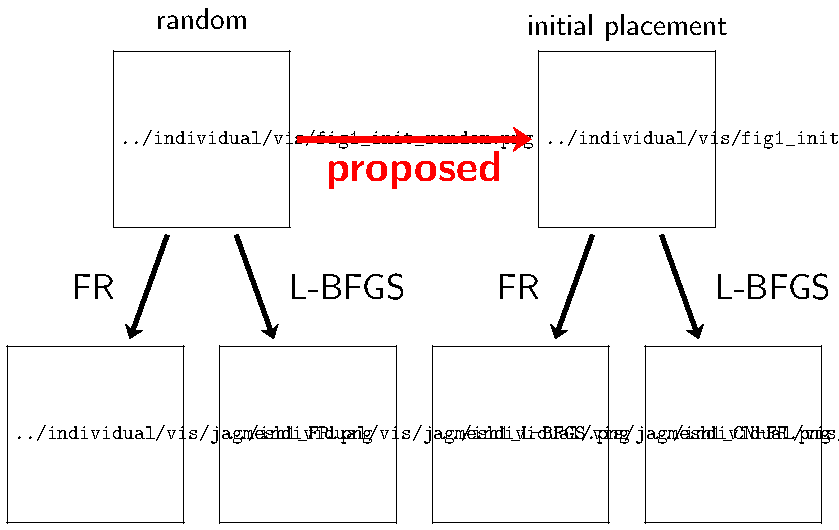
\includegraphics[width=0.8\columnwidth]{fig1/fig1_slide.pdf}
  \caption{Comparison of the algorithms for the \texttt{jagmesh1}.}
  \label{fig:fig1}
\end{figure}

Graph drawing is a fundamental task in information visualization, and force-directed methods are among the most widely used approaches. In these methods, vertices are treated as particles subject to forces, and the resulting equilibrium layouts are regarded as desirable visualizations.
Among established force models~\citep{eades1984heuristic,kamadaAlgorithmDrawingGeneral1989}, the Fruchterman--Reingold (FR) force model~\citep{fruchtermanGraphDrawingForcedirected1991} is particularly prominent for its intuitive formulation, flexibility, and simplicity. It is implemented in libraries such as NetworkX~\citep{hagbergExploringNetworkStructure2008}, Graphviz~\citep{ellsonGraphvizOpenSource2002}, and igraph~\citep{csardiIgraphSoftwarePackage2006}.

\red{Obtaining the equilibrium layout of the force models has been a subject of extensive research.} The FR algorithm~\citep{fruchtermanGraphDrawingForcedirected1991} is an original iterative method that simulates the forces to find an equilibrium, but it struggles with its scalability.
Its convergence becomes prohibitively slow on large graphs, prompting the development of multilevel coarsen-refine schemes such as the Scalable Force-Directed Placement (\textsf{sfdp}) method in Graphviz~\citep{Hu2006EfficientHF,ellsonGraphvizOpenSource2002}. While these frameworks extend the applicability, their refinement stage still relies heavily on the FR algorithm, leaving room for improvement.

The critical issue in the refinement step is that the twist slows down the force simulation. The term twist refers to unnecessary folded and tangled structures in the visualized graph~\cite{veldhuizenDynamicMultilevelGraph2007,cheongSnapshotVisualizationComplex2018}. The results in \cref{fig:fig1} highlight these twist issues. Even if a graph has a simple structure, twists often occur, which cancel out the forces and lead to stagnation and suboptimal visualization outcomes.

\red{To address the twist problem and obtain better equilibrium layouts, we utilize continuous optimization techniques.}
The L-BFGS algorithm~\citep{liuLimitedMemoryBFGS1989a} is a general purpose optimization algorithm and more practical approach~\citep{6183577}, \red{achieving better results for several force models including the FR force model and the Kamada--Kawai (KK) model~\citep{kamadaAlgorithmDrawingGeneral1989}.} % LLDisable
While L-BFGS algorithm can partially address the twist problem, it can require many iterations with high per-iteration cost.
It may fail to achieve optimal visualization within a limited number of iterations as shown in \cref{fig:fig1}.
A Stochastic Gradient Descent (SGD)-based method, which updates the positions of two vertices at a time based on a single edge, has recently been proposed for the KK layout.~\citep{zhengGraphDrawingStochastic2019,kamadaAlgorithmDrawingGeneral1989}.
While it is highly regarded, applying it to the force model in the FR algorithm is challenging due to its relatively complex structure.
Refer to \cref{sec:rationale} for more details.

Pre-processing to find a better initial placement is another optimization-based approach to solve the twist problem. A pre-processing step with Simulated Annealing (SA) is known to be effective since SA, the optimization method, can avoid getting stuck in local optima and leads to a better visualization combined with the FR algorithm~\cite{ghassemitoosiSimulatedAnnealingPreProcessing2016}. Still, as discussed in \cref{ssec:preprocessing}, this work focuses only on unweighted, simple-structured, and small-scale graphs.

In this paper, we propose a new initial placement for the force model in the FR algorithm. We provide an initial placement with fewer twists than random placement within a short time, accelerating the subsequent optimization process. We can use both FR and L-BFGS algorithms to obtain the final placement. This work extends the applicability of the initial placement idea to larger-scale, weighted, and complicated structured graphs. To achieve this, we optimize the position of vertices one by one with the coordinate Newton direction, leveraging the inherent structure and the sparsity of graphs. We also demonstrate its effectiveness through various experiments.

The remainder of the paper is organized as follows.
\begin{enumerate}[label=\textbullet, itemsep=0pt, parsep=0pt]
  \item In \cref{sec:preliminaries}, we provide the technical definitions of the FR force model. % LLDisable

  \item In \cref{sec:related_work}, we review some related work.

  \item In \cref{sec:algorithm}, we present our initial placement algorithm.

  \item In \cref{sec:experiment}, we report experimental comparisons.

  \item In \cref{sec:rationale}, we discuss our approach and its potential applications.

  \item In \cref{sec:conclusion}, we conclude the paper and discuss future work.
\end{enumerate}

\section{Preliminaries}
\label{sec:preliminaries}

Fruchterman and Reingold~\citep{fruchtermanGraphDrawingForcedirected1991}
proposed the FR algorithm with its force model for graph drawing based on the physical analogy of the system of particles. \red{Note that we distinguish between the FR algorithm and the FR model. The former is an iterative method that simulates the forces, while the latter is a mathematical formulation of the forces.}
Through the simulation of these forces, the FR algorithm seeks equilibrium positions.
In contrast to this ordinary approach, energy-based methods seek equilibrium.
A local minimum of the energy function $\Phi$ yields an equilibrium position since $\nabla \Phi(X)$ corresponds to the forces. In this sense, the force-based and energy-based perspectives are equivalent as both capture equilibrium, illustrated in \cref{fig:frLayout}.

\begin{figure}[t]
  \centering
  
\includegraphics[width=0.6\columnwidth]{fr_layout/fr_layout.pdf}
  \caption{ In the model, forces act on every pair of vertices. Forces $F_{i,j}
        ^{\mathrm{a}}(d)$ and $F^{\mathrm{r}}(d)$ work between vertices $i$ and $j$.
    The equilibrium of them is achieved at $d = k/\sqrt[3]{a_{i,j}}$, which equals $k$ when $a_{i,j}= 1$. }
  \label{fig:frLayout}
\end{figure}

Let us formally define the optimization problem for obtaining the equilibrium layout.
Let $G = (V, E)$ be an undirected graph with vertex set $V = \{1, \dots, n\}$ and edge set $E$. Each edge $\{i,j\} \in E$ has positive weight $a_{i,j} = a_{j,i} \in \mathbb{R}$.
For convenience, we set $a_{i,j}=0$ for $\{i, j\} \notin E$.
The force model in the FR algorithm assumes forces between vertices. For vertices $i$ and $j$ with distance
$d > 0$, an attractive force $F_{i,j}^{\mathrm{a}}(d)$ and a
repulsive force $F^{\mathrm{r}}(d)$ are defined as
\begin{equation*}
  F_{i,j}^{\mathrm{a}}(d) \coloneqq \frac{a_{i,j}d^{2}}{k}, \quad F^{\mathrm{r}}
  (d) \coloneqq -\frac{k^{2}}{d},
\end{equation*}
where $k > 0$ is a constant parameter, often set to $1/\sqrt{n}$~\citep{fruchtermanGraphDrawingForcedirected1991}.
The scalar potentials of these forces~\citep{6183577} are given by
\begin{gather*}
  \color{red}
  \Phi^{\mathrm{a}}_{i,j}(d) \coloneqq \int_{0}^{d}F_{i,j}^{\mathrm{a}}(r) \dd{r}= \frac{a_{i,j}d^{3}}{3k}, \quad
  \Phi^{\mathrm{r}}(d) \coloneqq \int_{1}^{d}F^{\mathrm{r}} (r) \dd{r}= -k^{2}\log{d}, \\
  \color{red}
  \Phi_{i,j}(d) \coloneqq \Phi_{i,j}^{\mathrm{a}}(d) + \Phi^{\mathrm{r}}(d).
\end{gather*}
For simplicity, we define $\Phi_{i,j}(0)=\infty$.%
\footnote{We can also use $-k^{2}\log(d + \epsilon^{\mathrm{r}})$ for $\Phi^{\mathrm{r}}
  (d)$ to prevent divergence, where $\epsilon^{\mathrm{r}}$ is constant.}
Let $\norm{\cdot}$ denote the Euclidean norm in $\mathbb{R}^{2}$. Then, the problem is to minimize the energy with
$X \coloneqq (x_{1}, \dots, x_{n}) \in \mathbb{R}^{2 \times n}$:
\begin{mini}
  {X \in \mathbb{R}^{2 \times n}} {\Phi(X) \coloneqq \sum_{\substack{(i,j) \in V^2 \\ i \neq j}} \Phi_{i,j}(\norm{x_i - x_j}).}
  {\label{prob:fr}} {}
\end{mini}
{\color{red} Note that the summation is taken over ordered pairs $(i,j)$.
For undirected graphs, this includes both $(i,j)$ and $(j,i)$ and therefore only scales the objective value by a constant factor.
We keep this form since it extends naturally to directed or asymmetric weights.}

While the energy function $\Phi_{i,j}(d)$ is convex and minimized when
$d = k/\sqrt[3]{a_{i,j}}$ for a positive $a_{i,j}$, a function $x_{i}\mapsto \Phi_{i,j}
  (\norm{x_i - x_j})$ is non-convex for a fixed $x_{j}$. Additionally, $\Phi_{i,j}$ is not Lipschitz continuous near $d=0$, as illustrated in \cref{fig:energy3d}.
These properties highlight the difficulty of the optimization problem.

\begin{figure}[t]
  \centering
  
\includegraphics[width=0.6\columnwidth]{energy_3d/energy_3d.png}
  \caption{The energy function $\Phi_{i,j}(\norm{x_i - x_j})$ for
  $x_{i}=(x_{i,1},x_{i,2})$, $x_{j}=(0,0), a_{i,j}= 1$, and $k = 1$.}
  \label{fig:energy3d}
\end{figure}

\section{Related Work}
\label{sec:related_work}

We next summarize the existing literature relevant to our work.

\subsection{Optimization Approach}
\label{sec:optimization_approach}

Optimization-based methods for graph drawing have been actively investigated. Representative approaches include GPU acceleration~\citep{gajdosParallelFruchtermanReingold2016}, machine learning techniques~\citep{tiezziGraphNeuralNetworks2024}, and multi-objective formulations~\citep{ahmedMulticriteriaScalableGraph2022a}. Among optimization-based approaches, our attention is on the underlying optimization algorithms itself. In this section, we review the L-BFGS algorithm.

The L-BFGS algorithm, a renowned and widely used optimization
method, consistently outperforms the original FR algorithm in speed
and layout quality~\citep{6183577}. It uses the function value and the gradient to find the local optima. We define the sum of terms associated with the vertex $x_{i}$ as $\Phi_{i}$, which is explicitly given by
\begin{equation*}
  \Phi_{i}(x_{i}) \coloneqq \sum_{j \in V \setminus \{i\}}\Big( \Phi_{i,j}(\norm{x_{i}- x_{j}}) + \Phi_{j,i}(\norm{x_{j}- x_{i}}) \Big).
\end{equation*}
The $i$-th column of the gradient $\nabla \Phi(X) \in \mathbb{R}^{2 \times n}$ is
\begin{align*}
  (\nabla \Phi(X))_{i} & \defeq \nabla \Phi_{i}(x_{i}) = \sum_{j \in V \setminus \{i\}}\left(\frac{(a_{i,j}+a_{j,i})\norm{ x_{i}- x_{j}}}{k}- \frac{2k^{2}}{\norm{ x_{i}- x_{j}}^{2}}\right) (x_{i}- x_{j}) \\
                    & = 2 \sum_{j \in V \setminus \{i\}}\left(\frac{a_{i,j}\norm{ x_{i}- x_{j}}}{k}- \frac{k^{2}}{\norm{ x_{i}- x_{j}}^{2}}\right) (x_{i}- x_{j}).
\end{align*}
The graph layout can be obtained as the result of optimization using the L-BFGS solver with the gradient described above. A common choice for the initial solution is a random placement of nodes within the bounding box
$\{(x_{i}^{(1)},x_{i}^{(2)}) \mathrel\mid 0 \leq x_{i}^{(1)}\leq 1, 0 \leq x_{i}
    ^{(2)}\leq 1\}$ \citep{2020SciPy-NMeth}.
However, when the input is highly twisted or otherwise ill-conditioned,
L-BFGS can suffer from large per-iteration costs: each iteration operates on the full set of coordinates, which limits its ability to untangle local geometric defects.

\red{todo. describe here.}

\subsection{Multilevel Approach}

\red{Multilevel approaches such as \textsf{sfdp}~\citep{Hu2006EfficientHF} in Graphviz are important prior work for obtaining the equilibrium layout of the force model, i.e., solving the problem~\eqref{prob:fr}.}
These methods use hierarchical coarsening and refinement to achieve efficient layout computation for large graphs.

Our work is complementary to such multilevel methods.
Optimization techniques such as L-BFGS can be directly applied to the refinement stages within multilevel pipelines. Since the approaches proposed in this study can be incorporated into multilevel frameworks with appropriate modifications, our primary objective is to quantify and enhance the refinement procedure itself.
Therefore, we deliberately exclude coarsening and other approximation steps from the present analysis.
For further details on multilevel approaches, the reader is referred to~\citep{harelFastMultiScaleMethod2002, walshawMultilevelAlgorithmForceDirected2003, arleoMultilevelApproachEventBased2021}.

\subsection{Initial Placement Approach}
\label{ssec:preprocessing}

A preprocessing step with Simulated Annealing (SA) is known to be effective~\citep{ghassemitoosiSimulatedAnnealingPreProcessing2016} since SA can avoid getting stuck in local optima and leads to better visualization, combined with the FR algorithm. Let
\begin{equation*}
  Q^{\mathrm{circle}} \defeq \left\{(\cos(2\pi i/n), \sin(2\pi i/n)) \mid 1 \leq i \leq n \right\}
\end{equation*}
be the points on a unit circle in $\bbR^{2}$. For an unweighted graph $G$, let
$E_{2}$ be a set of vertex pairs with a shortest path distance equal to 2. Let $\angle(a, b)$ denote the angle between the lines from the origin to the
points $a$ and $b$, measured in the interval $(-\pi, \pi]$. This study~\citep{ghassemitoosiSimulatedAnnealingPreProcessing2016}
defines the problem for the preprocessing of graph drawing as follows:
\begin{mini}
  {X \in \bbR^{2 \times n}} {\sum_{\{i,j\}\in E \cup E_2} \abs{\angle(x_i, x_j)},}
  {\label{eq:sa}} {} \addConstraint{x_i}{\in Q^\mathrm{circle} \quad}{\text{for $1 \leq i \leq n$}}
  \addConstraint{x_i}{\neq x_j \quad}{\text{for $1 \leq i < j \leq n$}.}
\end{mini}
The problem~\eqref{eq:sa} is a discrete optimization problem where the placement
is limited to $Q^{\mathrm{circle}}$ and uses angles, not the function $\Phi$ in
the problem~\eqref{prob:fr}. This study obtains a faster and better visualization by setting the
result of Simulated Annealing (SA) for the problem~\eqref{eq:sa} as an initial
placement for the FR algorithm.

Still, the following limitations remain:
\begin{enumerate}[label=\textbullet, itemsep=0pt, parsep=0pt]
  \item The target graphs are restricted to unweighted ones.

  \item The layout is confined to a simple circle, which could be ineffective
        for complex structured graphs.

  \item The neighborhood in the SA is the random swapping of two vertices,
        making the optimization process inefficient for large-scale graphs.

  \item $\abs{E_2}$ could be $\Theta(\abs{V}^{2})$, unable to leverage the
        sparsity of graphs if it exists.
\end{enumerate}
We address these limitations, and our study is an extension of this work.

\section{Proposed Algorithm}
\label{sec:algorithm}

With the prior studies in \cref{sec:optimization_approach}, this section proposes \cref{alg:proposed}, a new initial placement algorithm for
the problem~\eqref{prob:fr}. The algorithm solves a discrete optimization problem with stochastic coordinate descent to find an initial placement with fewer twists.
This algorithm leverages the properties of the objective function to determine the initial layout quickly. By combining it with optimization methods like the L-BFGS algorithm, it enhances the overall convergence speed of graph drawing through optimization.

\subsection{Newton Direction and Coordinate Newton Direction}
\label{ssec:introNewton}

Consider a strictly convex function $g \colon \bbR^{n}\to \bbR$ at $x_{0}$.
The Newton direction $d = -\nabla^{2}g(x_{0})^{-1}\nabla g(x_{0})$ is an
optimal direction for the second order approximation of $g$:
\begin{equation*}
  g(x_{0}) + \nabla g(x_{0})^{\top}(x - x_{0}) + \frac{1}{2}(x - x_{0})^{\top}\nabla
  ^{2}g(x_{0}) (x - x_{0}).
\end{equation*}
$x = x_{0}+ d$ is the minimizer of this approximation. Note that the Hessian
matrix $\nabla^{2}g(x_{0})$ is positive definite since $g$ is strictly convex.
Although the Newton direction is essential in various iterative methods, it
requires the computation of the inverse Hessian
$\nabla^{2}g(x_{0})^{-1}\in \bbR^{n \times n}$, posing a high computational cost
for large-scale problems.

Still, we can leverage the concept of the Newton direction in a different
manner, the coordinate Newton direction. Instead of computing the inverse
Hessian $\nabla^{2}g(x_{0})^{-1}$ in the entire variable space $\bbR^{n}$, we restrict
the variable $x$ to its coordinate block $x_{i}$ with fewer dimensions, and
compute $\nabla^{2}g_{i}(x_{i})^{-1}\nabla g_{i}(x_{i})$ where $g_{i}$ is a
restricted function of $g$ to $x_{i}$. Since the coordinate Newton direction computation
is much cheaper than that of the Newton direction, we can repeat this
procedure many times. In general, this idea is known as stochastic coordinate
descent~\citep{wright2022optimization} or Randomized Subspace Newton~\citep{NEURIPS2019_bc6dc48b}
in a broader context.

In particular, this coordinate Newton direction has an apparent natural affinity
to the problem~\eqref{prob:fr}. We can compute the coordinate
Newton direction by taking the position $x_{i}$ of the vertex $i$ as the coordinate
block. Although directly applying this idea to the problem~\eqref{prob:fr} is challenging,
as we will discuss in \cref{sec:rationale}, we leverage this coordinate Newton
direction to propose our algorithm.

\subsection{Discrete Optimization Problem for Initial Placement}
\label{ssec:reduction}

Even at the expense of accuracy, obtaining an approximate solution quickly is crucial
for the initial placement. To obtain it, we simplify the problem~\eqref{prob:fr}
into a more manageable and well-behaved discrete optimization problem:
\begin{mini}
  {X \in \bbR^{2 \times n}} {\Phi^\mathrm{a}(X) \defeq \sum_{\{i,j\}\in E} \frac{a_{i,j}\norm{x_i - x_j}^{3}}{3k},}
  {\label{eq:frApprox0}} {} \addConstraint{x_i}{\in Q^\mathrm{hex} \quad}{\text{for $1 \leq i \leq n$}}
  \addConstraint{x_i}{\neq x_j \quad}{\text{for $1 \leq i < j \leq n$},}
\end{mini}
where
\begin{equation}
  \label{eq:qHex}Q^{\mathrm{hex}}\defeq \left\{ \qty(q+\frac{1}{2}r, \frac{\sqrt{3}}{2}
  r) \relmiddle| q \in \bbZ,\ r \in \bbZ \right\}.
\end{equation}

\begin{figure}[t]
  \centering
  
\includegraphics[width=0.7\columnwidth]{pi/pi.pdf}
  \caption{ Concept of $Q$. The assignment from $V$ to a discrete point
    placement $Q$, especially a hexagonal lattice $Q^{\mathrm{hex}}$.
    Apparently, among the three placements, the right one is the best
    placement for the problem~\eqref{eq:frApprox0}. }
  \label{fig:pi}
\end{figure}

First, the problem~\eqref{prob:fr} is equivalent to the following:
\begin{mini*}
  {X \in \bbR^{2 \times n}} {\sum_{\{i,j\}\in E} \frac{a_{i,j}\norm{x_i - x_j}^{3}}{3k}- \sum_{i<j} k^2\log{\norm{x_i - x_j}}.}
  {} {}
\end{mini*}
This formulation separates the $\order{\abs{E}}$ terms from
$\Phi^{\mathrm{a}}_{i,j}$ and the $\order*{\abs{V}^2}$ terms from
$\Phi^{\mathrm{r}}$.

Here, following previous research mentioned in \cref{ssec:preprocessing}, we
fix the possible positions $x_{i}$ of each vertex $i$ to a discrete set of
points $Q$, where $\abs{Q}\geq \abs{V}$. It means that we consider the
following:
\begin{mini*}
  {X \in \bbR^{2 \times n}} {\sum_{\{i,j\}\in E} \frac{a_{i,j}\norm{x_i - x_j}^{3}}{3k}- \sum_{i<j} k^2\log{\norm{x_i - x_j}},}
  {} {} \addConstraint{x_i}{\in Q \quad}{\text{for $1 \leq i \leq n$}}
  \addConstraint{x_i}{\neq x_j \quad}{\text{for $1 \leq i < j \leq n$}.}
\end{mini*}
The goal is to simplify the objective function and choose $Q$ appropriately to
derive a well-simplified problem.

Due to the sparsity of many practical graphs, $\abs{E}\ll \abs{V}^{2}$ holds. To leverage this sparsity for simplification, we want to drop the second term
that arises from the repulsive energy $\Phi^{r}$:
\begin{equation*}
  -\sum_{i<j}k^{2}\log{\norm{x_i - x_j}}.
\end{equation*}
We impose a condition on $Q$ such that $\norm{q_{i}- q_{j}}\geq \epsilon$ for all
$q_{i}, q_{j}\in Q$ with $q_{i}\neq q_{j}$. In this case, the term above is negligible.
Since $\Phi^{\mathrm{r}}(d)=-k^{2}\log{d}$ is a convex function such that it
decreases monotonically concerning $d$, for sufficiently large $d$, the value
of $-k^{2}\log{d}$ does not vary excessively. For too small $d$, we can
prevent the divergence of the energy function by setting $\epsilon$. Thus, under this condition, we drop the second term and derive the problem as:
\begin{mini*}
  {X \in \bbR^{2 \times n}} {\sum_{\{i,j\}\in E} \frac{a_{i,j}\norm{x_i - x_j}^{3}}{3k},}
  {} {} \addConstraint{x_i}{\in Q \quad}{\text{for $1 \leq i \leq n$}}
  \addConstraint{x_i}{\neq x_j \quad}{\text{for $1 \leq i < j \leq n$}.}
\end{mini*}
This means that we skip to consider the $\order*{\abs{V}^2}$ pairs (all pairs of
$\{i,j\}$ with $1 \leq i < j \leq n$) by fixing the possible point placement
in advance, reducing the computational complexity to $\order{\abs{E}}$ and thus
offering significant speedup. See \cref{fig:pi} for a visual explanation.

We can consider various placements for the $Q$, including $Q^{\mathrm{circle}}$~\citep{ghassemitoosiSimulatedAnnealingPreProcessing2016}.
In this study, we adopt a hexagonal lattice $Q^{\mathrm{hex}}$~\citep{patelHexagonalGrids2013,s22145179}
defined by~\cref{eq:qHex} (see \cref{fig:pi}). When minimizing the objective
function that arises from the attractive energy $\Phi^{\mathrm{a}}$, it is advantageous
for the points to cluster as closely as possible. In this context, the hexagonal
lattice is known for its densest packing structure in space with the least distance
$\epsilon$ between points \citep{changSimpleProofThues2010} and offers
computational simplicity. Thus, $Q^{\mathrm{hex}}$ is a suitable choice, and we
have derived the problem~\eqref{eq:frApprox0}.

\subsection{Newton Direction for Discrete Optimization}
\label{ssec:newtonDirection}

Next, we solve the discrete optimization problem~\eqref{eq:frApprox0}.
Although this problem is challenging to solve just using simple methods, the coordinate Newton direction of a randomly selected vertex $i$ provides significant insights
as mentioned in \cref{ssec:introNewton}. Therefore, we can offer a high-quality
solution to the problem. Let the restricted objective function
$\Phi^{\mathrm{a}}_{i}(x_{i})$ be
\begin{equation*}
  \Phi^{\mathrm{a}}_{i}(x_{i}) \defeq \sum_{j \in V \setminus \{i\}}\frac{a_{i,j}\norm{x_i - x_j}^{3}}{3k}
  .
\end{equation*}
Its gradient and Hessian matrix are
\begin{align*}
  \nabla \Phi^{\mathrm{a}}_{i}(x_{i})    & = \sum_{j \in V \setminus \{i\}}\frac{a_{i,j}\norm{x_i - x_j}}{k}(x_{i}- x_{j}),                                        \\
  \nabla^{2}\Phi^{\mathrm{a}}_{i}(x_{i}) & = \sum_{j \in V \setminus \{i\}}\frac{a_{i,j}\norm{x_i - x_j}}{k}\mqty(1                                            & 0 \\
  0                                   & 1) + \sum_{j \in V \setminus \{i\}}\frac{a_{i,j}}{k\norm{x_i - x_j}}(x_{i}- x_{j})(x_{i}- x_{j})^{\top}.
\end{align*}
This means $\Phi^{\mathrm{a}}_{i}$ is strictly convex, assuring the Hessian matrix
$\nabla^{2}\Phi^{\mathrm{a}}_{i}(x_{i})$ is positive definite. This is a large
difference from the functions $\Phi(X)$ in the problem~\eqref{prob:fr} and $\Phi^{\mathrm{a}}
  (X)$ in the problem~\eqref{eq:frApprox0}, which are non-convex.

The ordinary updated rule with the coordinate Newton direction is
\begin{equation*}
  x_{i}^{\mathrm{new}}\gets x_{i}- \nabla^{2}\Phi^{\mathrm{a}}_{i}(x_{i})^{-1}\nabla
  \Phi^{\mathrm{a}}_{i}(x_{i}).
\end{equation*}
$x_{i}^{\mathrm{new}}$ may not be in the hexagonal lattice $Q^{\mathrm{hex}}$ in
the problem~\eqref{eq:frApprox0}. Thus, we project this $x_{i}^{\mathrm{new}}$
onto the nearest point in $Q^{\mathrm{hex}}$. We also empirically found that adding a random noise vector to the Newton direction is effective for the optimization
process, a strategy similar to the SA in \cref{ssec:preprocessing}. This randomness can help to escape from local minima and to explore the solution space more effectively.
In conclusion, the updated rule for the vertex $i$ is
\begin{equation*}
  x_{i}^{\mathrm{new}}\gets \mathrm{round}\qty(x_{i}- \nabla^{2}\Phi^{\mathrm{a}}_{i}
  (x_{i})^{-1}\nabla \Phi^{\mathrm{a}}_{i}(x_{i}) + t \cdot r),
\end{equation*}
where $\mathrm{round}(\hat{x})$ denotes the operation assigning $\hat{x}$ to the
nearest point in the hexagonal lattice $Q^{\mathrm{hex}}$, $r$ is a random vector with a unit norm, and the parameter $t$ is gradually decreased as the iterations
proceed and is designed to converge to zero eventually.

If there is a vertex $j$ such that $x_{j}= x_{i}^{\mathrm{new}}$, we swap the
positions $x_{i}$ and $x_{j}$ to satisfy the condition $x_{i}\neq x_{j}$. Otherwise,
we just update $x_{i}$ to $x_{i}^{\mathrm{new}}$. Refer to \cref{fig:hex} for a
visual explanation. Repeating this procedure yields an approximate solution to
the problem~\eqref{eq:frApprox0}.

\begin{figure}[t]
  \centering
  
\includegraphics[width=0.7\columnwidth]{hex/hex.pdf}
  \caption{One iteration of the proposed algorithm. Step 1. Compute the coordinate
    Newton direction (blue). Step 2. Decide $x_{i}^{\mathrm{new}}$ by rounding the direction and adding a random vector. Step 3. Move the vertex and swap the vertices if necessary (swap blue and green vertices).}
  \label{fig:hex}
\end{figure}

\subsection{Optimal Scaling}
\label{ssec:optimalScaling}

The obtained solution could be too small or too large since we did not care
about the scale $\epsilon$. Thus, as the final step, we rescale the placement to
improve it.

Let us formulate the optimization problem for the scaling factor $s > 0$. For
an initial placement $X = (x_{1}, \dots, x_{n})$, we scale it as $x_{i}\gets s
  x_{i}$ for all $i$. The problem of minimizing $\Phi(X)$ through scaling is
equivalent to minimizing $\phi(s)$ defined by
\begin{align*}
  \phi(s) \defeq{} & \sum_{\{i,j\} \in E}\frac{a_{i,j}(s \norm{x_i - x_j})^{3}}{3k}- k^{2}\sum_{i < j}\log(s \norm{x_i - x_j}), \\
  \phi'(s) ={}     & \sum_{\{i,j\} \in E}\frac{a_{i,j}\norm{x_i - x_j}^{3}}{k}s^{2}- \frac{k^{2}n(n-1)}{2s}.
\end{align*}
The function $\phi(s)$ is convex, and the optimal scaling factor $s^{*}$ satisfies
$\phi'(s^{*}) = 0$, which yields
\begin{equation}
  \label{eq:scaling}s^{*}= \qty(\frac{k^{3}n(n-1)}{2 \sum_{\{i,j\} \in E}a_{i,j}\norm{x_i - x_j}^{3}}
  )^{1/3}.
\end{equation}
This value can be computed in $\order{\abs{E}}$ complexity, enabling us to obtain
a better initial placement for the problem~\eqref{prob:fr}.

Notably, the optimal solution to the problem~\eqref{eq:frApprox0} is invariant
under scaling. Thus, we do not have to care about the scale factor for the
hexagonal lattice $Q^{\mathrm{hex}}$ as far as we scale the obtained placement
by $s^{*}$.

\begin{algorithm}
  [ht]
  \caption{Proposed algorithm for the initial placement}
  \label{alg:proposed} \KwIn{Graph $G = (V, E)$, Weight $(a_{i,j})_{\qty{i,j} \in E}$, Parameters $N_{\mathrm{iter}}^{\mathsf{CN}}\in\bbN,$ and $t_{0}>0$}
  \KwOut{Initial placement $X = (x_{1}, \dots, x_{n})$} $t \gets t_{0}$\;
  Sample $x_{i}\in Q^{\mathrm{hex}}$ for all $i \in V$ without replacement\;
  \For{$m \gets 0$ \KwTo $N_{\mathrm{iter}}^{\mathsf{CN}}$}{
    Select vertex $i \in V$ randomly\;
    Draw $r \in \bbR^{2}$ randomly from a unit circle\;
    $x_{i}^{\mathrm{new}}\gets \mathrm{round}(x_{i}- \nabla^{2}\Phi_{i}^{\mathrm{a}}(x_{i})^{-1}\nabla \Phi_{i}^{\mathrm{a}}(x_{i}) + t \cdot r)$\;
    \If{$\exists j \in V$ such that $x_{j}= x_{i}^{\mathrm{new}}$}{
      % Swap $x_i$ and $x_j$\;
      $x_{j}\gets x_{i}$\;
    }
    $x_{i}\gets x_{i}^{\mathrm{new}}$\; $t \gets t - t_{0}/ N_{\mathrm{iter}}^{\mathsf{CN}}$\;
  }
  $x_{i}\gets s^{*}x_{i}$ for all $i \in V$ with $s^{*}$ given by \cref{eq:scaling}\;
  \Return $X$
\end{algorithm}

\subsection{Alternative Approach}
\label{ssec:alternative}

To end this section, we explain an alternative approach to the problem~\eqref{eq:frApprox0}.
We can also solve the problem by updating all vertices simultaneously, not one
by one. It means moving all the points $\{x_{i}\}_{i \in V}$ to arbitrary positions
and then assigning all these $\abs{V}$ points to the nearest points on $Q^{\mathrm{hex}}$.
The optimal assignment for $\{x_{i}\}_{i \in V}$ to $Q^{\mathrm{hex}}$ is
computable by a Hungarian algorithm in $\order*{\abs{V}^3}$ time or some
heuristic.

{
  \color{red}

  \subsection{Application to Other Force Models}

We briefly discuss and explore the potential applicability of stochastic coordinate descent to a broader range of problems.
Although we utilized the coordinate Newton direction only for the optimization problem~\eqref{prob:fr}, we can see that its application is not necessarily limited to the FR force model, the problem~\eqref{prob:fr}. % LLDisable

Recall that Our optimization problem~\eqref{prob:fr} can be rewritten as
\begin{mini*}
  {X \in \bbR^{2 \times n}} {\Phi_{\mathrm{FR}}(X) = \sum_{(i,j)\in E} \frac{a_{i,j}\norm{x_{i} - x_{j}}^{3}}{3k} - \sum_{\substack{(i,j) \in V^2 \\ i \neq j}} k^2\log{(\epsilon^{\mathrm{r}} + \norm{x_{i} - x_{j}})}.}
  {} {}
\end{mini*}
Similar objective functions arise from other force models, such as ... are as follows:
\begin{mini*}
  {X \in \bbR^{2 \times n}} {
  \Phi_{\mathrm{HC}}(X) =
\sum_{(i,j)\in E \land j>i}
\frac{k_1(\lVert x_{i} - x_{j} \rVert - a_{ij})^2}{2}
+
\sum_{\substack{(i,j) \in V^2 \\ i \neq j}}
\frac{k_2}{\lVert x_{i} - x_{j} \rVert + \epsilon^{\mathrm{r}}}}{}{}
\end{mini*}
\begin{mini*}
  {X \in \bbR^{2 \times n}} {\Phi_{\mathrm{Eades}}(X) =
\sum_{(i,j)\in E}
k_1 \lVert x_{i} - x_{j} \rVert
\left(
\log \frac{\lVert x_{i} - x_{j} \rVert}{a_{ij}} - 1
\right)
+
\sum_{\substack{(i,j) \in V^2 \\ i \neq j}}
\frac{k_2}{\lVert x_{i} - x_{j} \rVert + \epsilon^{\mathrm{r}}}}{}{}
\end{mini*}
Clearly, these objective functions are also non-convex and have a similar structure to $\Phi_{\mathrm{FR}}(X)$, which consists of a sum of terms associated with edges and a sum of terms associated with all pairs of vertices. The coordinate Newton direction can be computed for each vertex in these models as well, and the stochastic coordinate descent approach can be applied to optimize the layout efficiently.

% なお、より広い枠組みとして、stochastic coordinate descentは、グラフから生じる目的関数に対して、各頂点の位置を座標ブロックとして取ることで適用できます~\citep{wright2022optimization}。
% それ故にKK modelに対しても同様のアプローチが可能であると考えられます。
% しかし、提案手法をそのままapplyすることは難しいと考えています。
% KK modelの目的関数は、以下の通りです。
\begin{mini*}
  {X \in \bbR^{2 \times n}} {\Phi_{\mathrm{KK}}(X) \coloneqq \sum_{\substack{(i,j) \in V^2 \\ i \neq j}}  \frac{(\lVert p_{ij} \rVert - l_{ij})^2}{2 l_{ij}^2}}
  {} {}
\end{mini*}
% 実際、これは先ほどまでにあげた目的関数と同様の構造を持っていますが、KK modelの目的関数は、すべての頂点ペアに対して項が存在するため、計算コストが高くなります。
}

\section{Numerical Experiment}
\label{sec:experiment}

In this section, we evaluate the proposed algorithm with various numerical
experiments. We also confirm that the proposed algorithm efficiently provides a
good initial placement even for larger weighted graphs.

\subsection{Experimental Setup}
\label{ssec:setup}

We conducted all numerical experiments in this section using \Cpp{17} compiled
by GCC 10.5.0 on a laptop computer powered by Intel(R) Core(TM) i7-10510U CPU
with \SI{16}{\giga\byte} RAM.

For a fair comparison, we implemented the FR algorithm in \Cpp{} based on
NetworkX version 3.3~\citep{hagbergExploringNetworkStructure2008}, SciPy 1.14.1~\citep{2020SciPy-NMeth},
and utilized the \Cpp{} L-BFGS~\citep{qiuYixuanLBFGSpp2024,okazakiChokkanLiblbfgs2024}
library for the L-BFGS algorithm. We also referred to the open-source code of the hexagonal grid~\citep{patelHexagonalGrids2013} and Graphviz version 2.43.0~\citep{ellsonGraphvizOpenSource2002}.

We used the $3 \times 2$ algorithms. As an initial placement, we used
\begin{enumerate}[label=\textbullet, itemsep=0pt, parsep=0pt]
  \item random initialization (no prefix),

  \item the SA initialization obtained by Simulated Annealing (\textsf{SA-})~\citep{ghassemitoosiSimulatedAnnealingPreProcessing2016},

  \item the proposed initialization obtained with coordinate Newton direction (\textsf{CN-}).
\end{enumerate}
As an algorithm to solve the problem~\eqref{prob:fr}, we used
\begin{enumerate}[label=\textbullet, itemsep=0pt, parsep=0pt]
  \item FR algorithm (\textsf{FR}),

  \item L-BFGS algorithm (\textsf{L-BFGS}).
\end{enumerate}
\red{The key remark is that we slightly modified the FR algorithm so that it automatically adjust the stepsize. This is to isolate the effect of the proposed initialization from the effect of the stepsize. This is just done by a simple backtracking line search at the first iteration.}

\begin{figure*}[p]
  
\includegraphics[width=\columnwidth]{individual/individual.pdf}
  \makebox[\columnwidth][r]{%
    \makebox[0.8\columnwidth][c]{%
      
\includegraphics[width=0.5\columnwidth]{individual/legend.pdf}
    }%
  }
  \caption{
    Experimental results. Our proposed method \textsf{CN}, Coordinate Newton, yields improved results for both FR and L-BFGS.
    The ``BEST'' reports the performance of \textsf{CN-L-BFGS} within at most 500 iterations.
    \red{The color of vertices represents their indices.}
  }
  \label{fig:individual}
\end{figure*}

As parameters, we used initial temperature $t_{0}=1.5$ and the number of
iterations $N_{\mathrm{iter}}^{\mathsf{CN}}= 2 \abs{V}^{3}/ \abs{E}$ for~\cref{alg:proposed}, and we also set the total number of iterations of Simulated Annealing (\textsf{SA}) in~\cref{ssec:preprocessing} to the same value.
Since the \cref{alg:proposed} requires a computational time proportional to the degree of the selected vertex in each iteration, the expected computational time per iteration is $\order*{\abs{E}/\abs{V}}$.
Consequently, we can roughly estimate that the total computational time of the proposed algorithm is $\order*{\abs{V}^2}$, equivalent to a few iterations of the FR or L-BFGS algorithms.
All the codes are available at GitHub~\citep{ThisPaperGitHub}.

\begin{figure*}[t]
  \centering
  \begin{minipage}{0.475\columnwidth}
    \centering
    
\includegraphics[width=\columnwidth]{overall/plot/diff_FR_50.pdf}
  \end{minipage}
  \hfill
  \begin{minipage}{0.475\columnwidth}
    \centering
    
\includegraphics[width=\columnwidth]{overall/plot/diff_L-BFGS_50.pdf}
  \end{minipage}
  \caption{ Comparison of the proposed initialization (\textsf{CN}) with
    random initialization (no prefix). In almost all cases, the difference is
    negative, meaning the proposed algorithm performed faster and better than random
    initialization. }
  \label{fig:overall}
\end{figure*}
\begin{figure*}[!t]
  \centering
  \begin{minipage}{0.475\columnwidth}
    \centering
    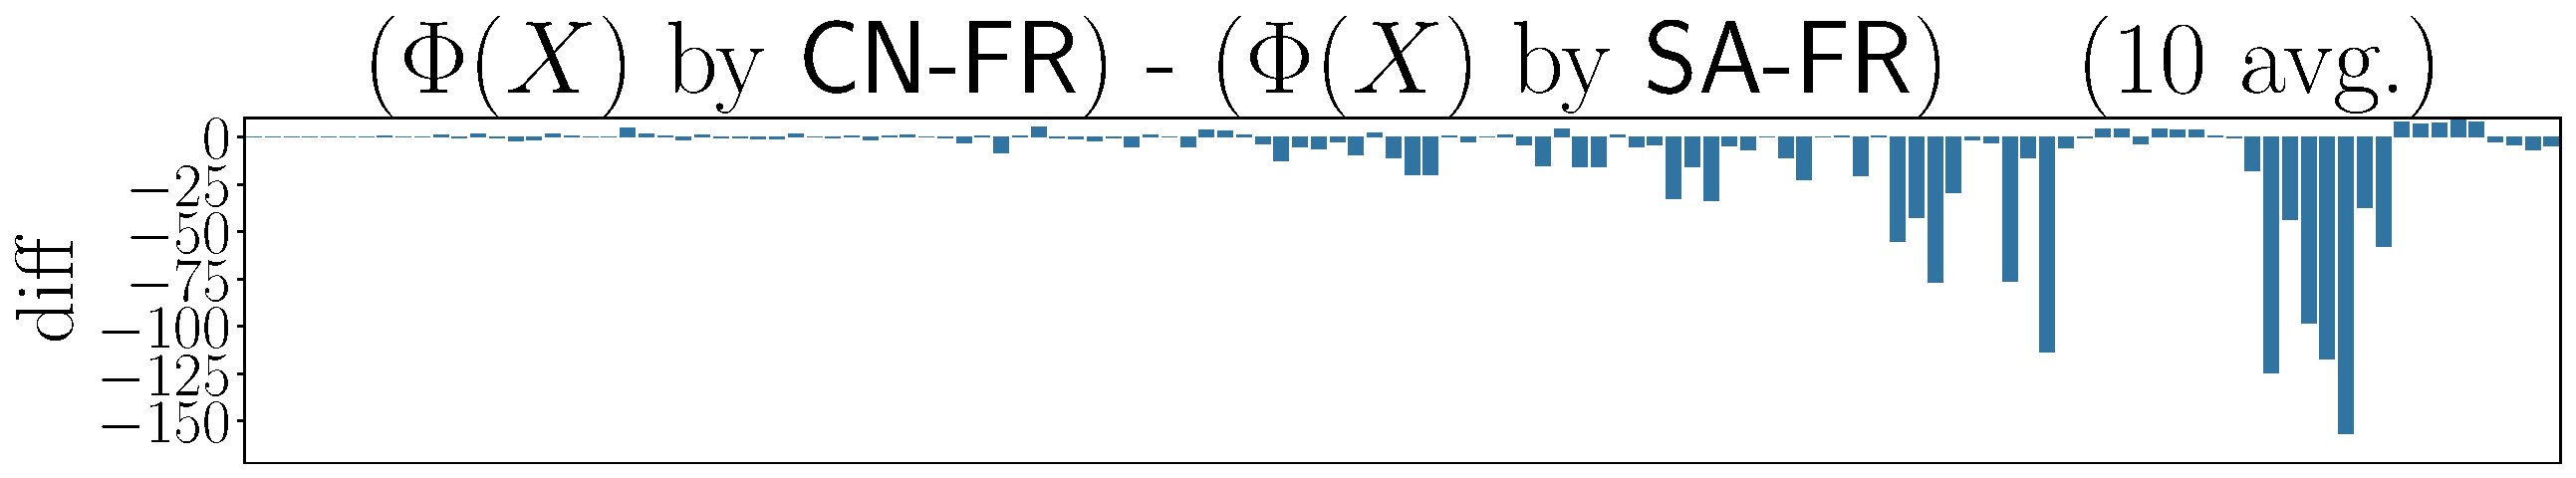
\includegraphics[width=\columnwidth]{circle/plot/diff_FR_50.pdf}
  \end{minipage}
  \hfill
  \begin{minipage}{0.475\columnwidth}
    \centering
    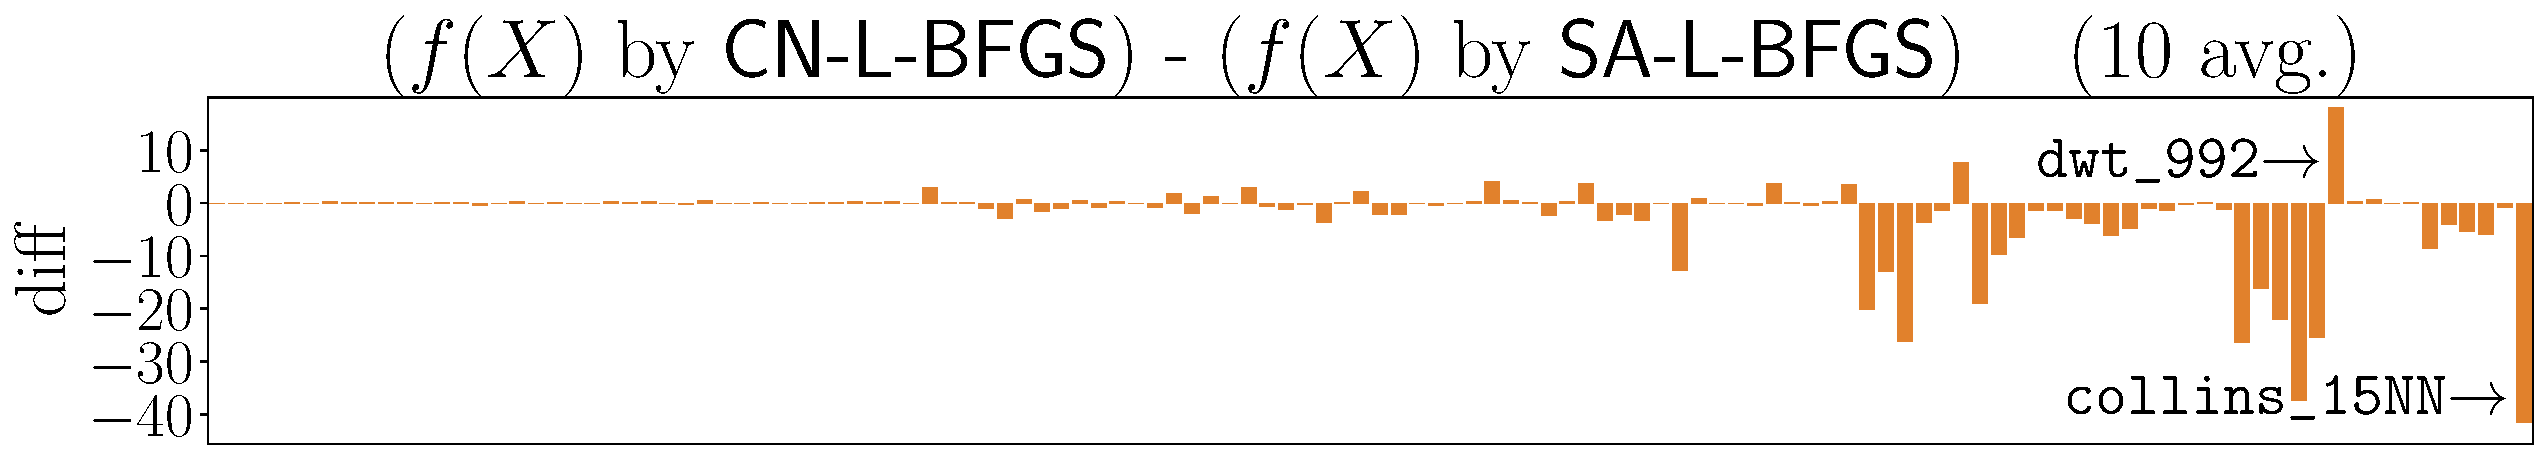
\includegraphics[width=\columnwidth]{circle/plot/diff_L-BFGS_50.pdf}
  \end{minipage}
  \caption{ Comparison of the proposed initialization (\textsf{CN}) with SA
    initialization (\textsf{SA}) in Ref.~\citep{ghassemitoosiSimulatedAnnealingPreProcessing2016}.
    In most cases, the proposed algorithm performed better than the SA initialization.
  }
  \label{fig:diff}
\end{figure*}
\begin{figure*}[t]
  \centering
  \begin{minipage}{\columnwidth}
    \centering
    \begin{minipage}{0.32\columnwidth}
      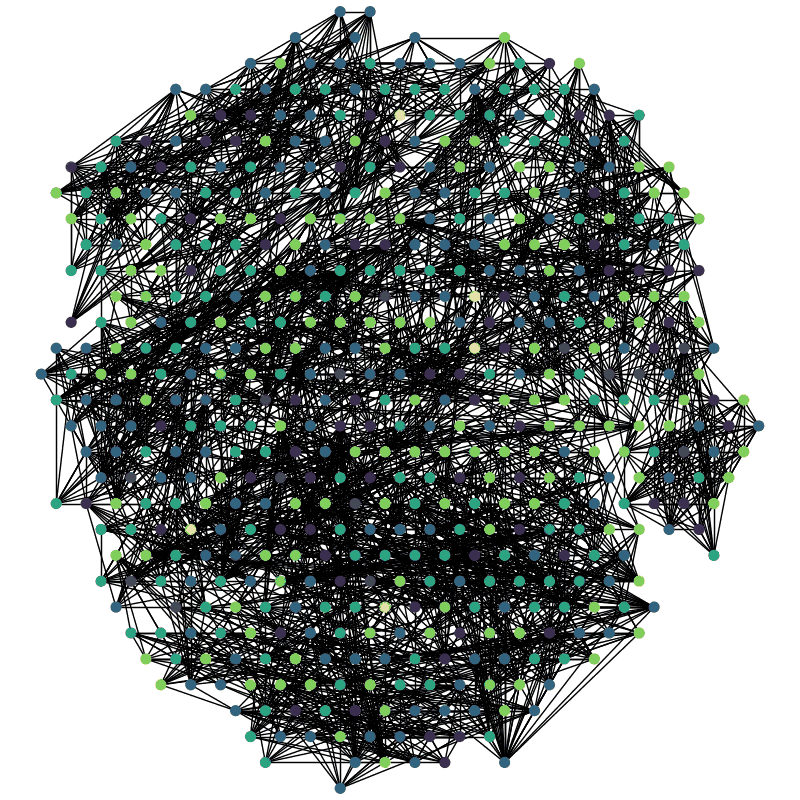
\includegraphics[height=2.8cm]{
        overall/vis/Spectro_10NN_CN-L-BFGS_50_first.png
      }
    \end{minipage}
    \begin{minipage}{0.32\columnwidth}
      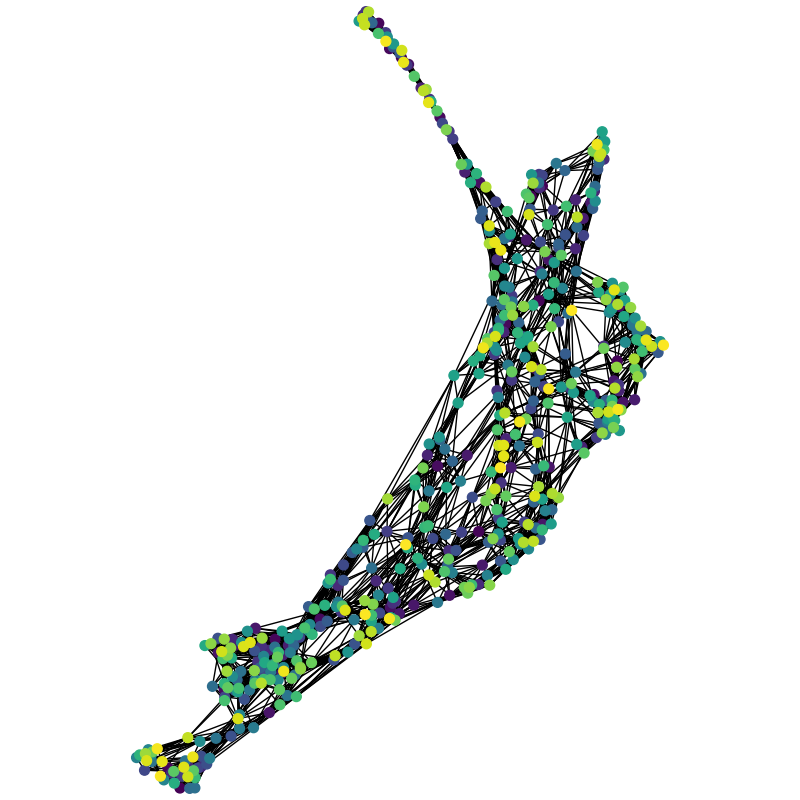
\includegraphics[height=2.8cm]{
        overall/vis/Spectro_10NN_CN-L-BFGS_50_last.png
      }
    \end{minipage}
    \begin{minipage}{0.32\columnwidth}
      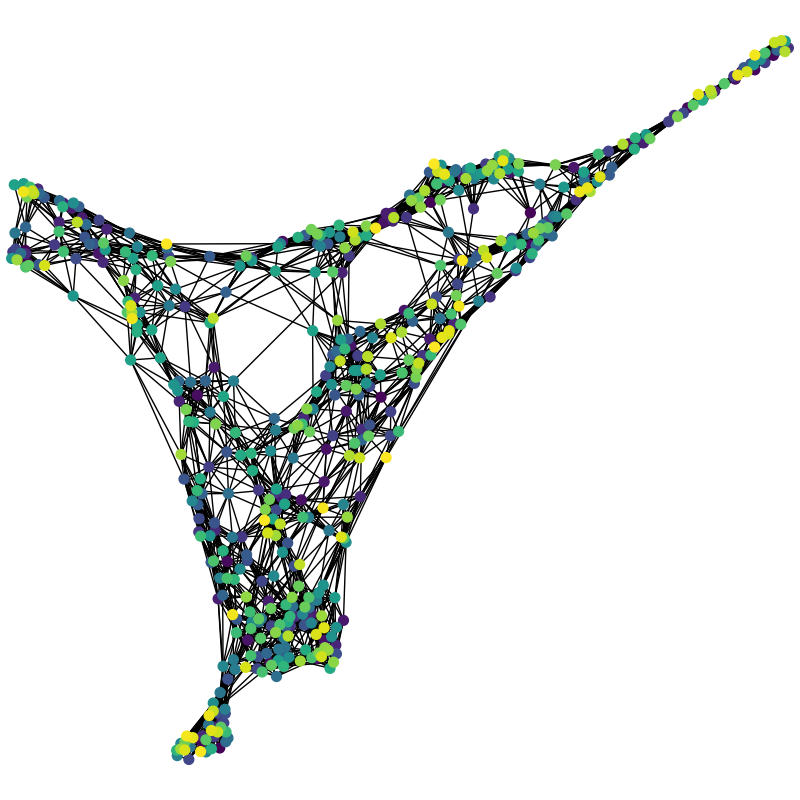
\includegraphics[height=2.8cm]{
        overall/vis/Spectro_10NN_CN-L-BFGS_50_final.png
      }
    \end{minipage}
    \caption{ \texttt{Spectro\_10NN}, where the proposed algorithm performed worse
      than random initialization. Left: Initial placement by \textsf{CN}. Middle
      and Right: 50th and 200th iteration of \textsf{CN-L-BFGS}. }
    \label{fig:proposeIsBad}
  \end{minipage}
  \hfill
  \begin{minipage}{\columnwidth}
    \centering
    \begin{minipage}{0.4\columnwidth}
      \centering
      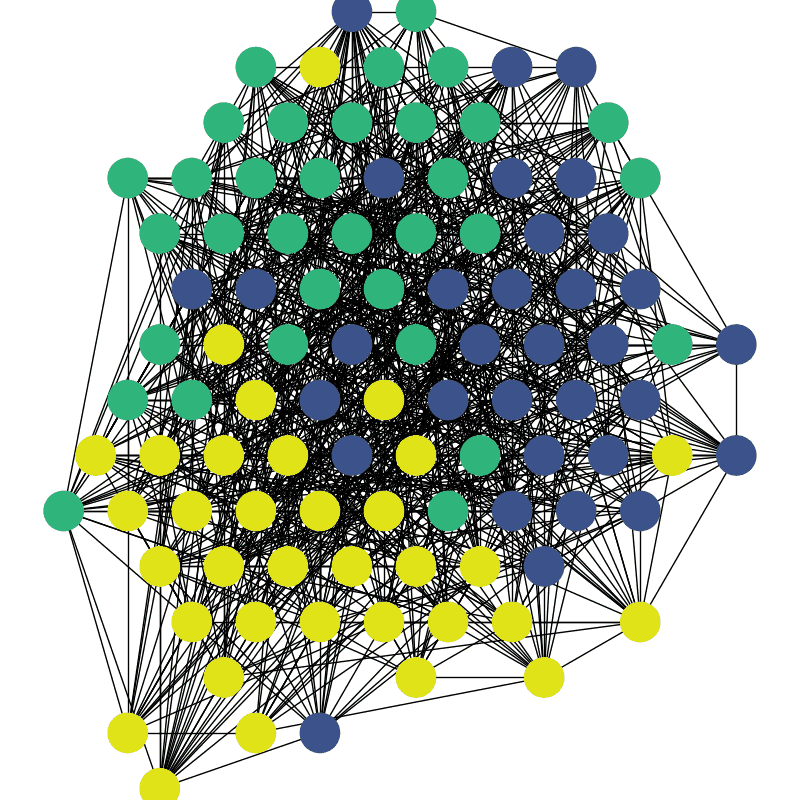
\includegraphics[height=2.8cm]{circle/vis/dense_CN-L-BFGS_10.png}
    \end{minipage}
    \begin{minipage}{0.4\columnwidth}
      \centering
      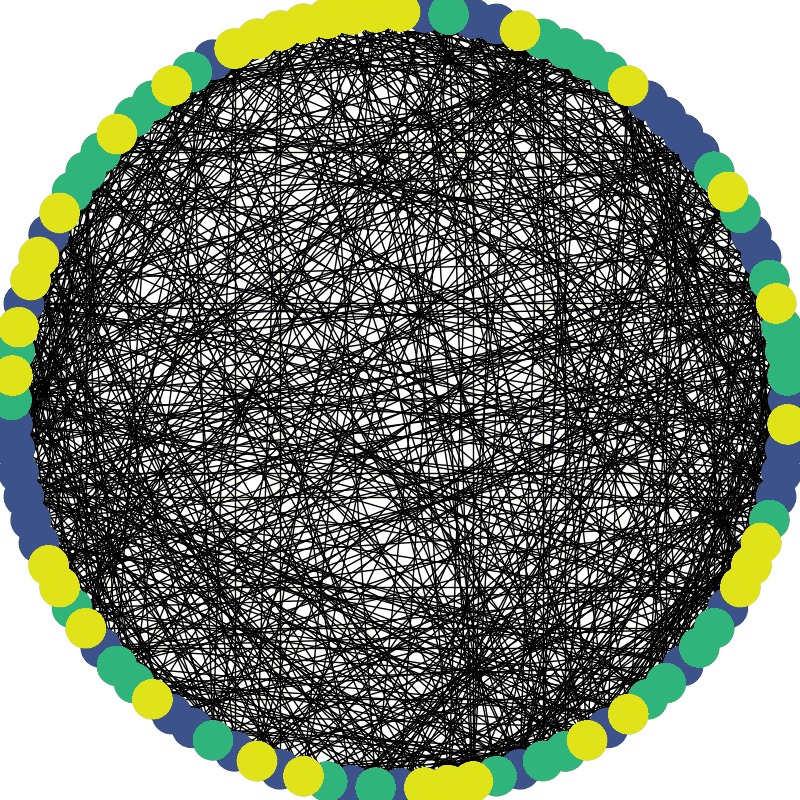
\includegraphics[height=2.8cm]{circle/vis/dense_SA-L-BFGS_10.png}
    \end{minipage}
    \caption{ An example of a case where $a_{i,j}\notin \{0,1\}$. Left: the result
      of \textsf{CN}, which is better as the vertices are separated by colors.
      Right: the result of \textsf{SA}, which is worse as there is no separation.
    }
    \label{fig:weightedDense}
  \end{minipage}
\end{figure*}

\subsection{Plots and Visualizations}
\label{ssec:exprDetail}

We first show the plots and visualizations of the algorithms in \cref{fig:individual}.
The experiment details are as follows. We fixed the maximum number of iterations
of the FR and L-BFGS algorithms as $N_{\mathrm{iter}}^{\mathsf{FR}}= N_{\mathrm{iter}}
  ^{\mathsf{LBFGS}}= 200$. We tested with 7 graphs: \texttt{cycle300}, \texttt{jagmesh1},
\texttt{dwt\_1005}, \texttt{btree9}, \texttt{1138\_bus}, \texttt{dwt\_2680}, and
\texttt{3elt}. Here \texttt{cycle300} is a cycle graph with 300 vertices, and \texttt{btree9}
is a perfect binary tree with $2^{9+1}-1=1023$ vertices.
Other graphs are from Sparse Matrix Collection~\citep{davisUniversityFloridaSparse2011}, and these choices are based on Ref.~\citep{zhengGraphDrawingStochastic2019}.

In \cref{fig:individual}, the plots on the left illustrate the objective function values $\Phi(X)$, the average of the ten trials for each algorithm.
The graphs on the right are at the iteration in which the most significant difference appeared among \{50,100,150\}-th iterations (or at the last iteration if it ended earlier).
The vertices in the graphs are colored according to vertex indices.

The observations and implications of \cref{fig:individual} are as follows.
First, the plots with solid lines for \textsf{CN} generally demonstrate superior performance to those with dashed lines for non-\textsf{CN}.
These results validate the efficacy of the proposed method.
Secondly, the initial values of $\Phi(X)$ with \textsf{CN-FR} are significantly smaller than those with \textsf{FR}, suggesting that the proposed method provides a good initial placement.
Thirdly, the visualization results also support the effectiveness of the proposed initial placement. In most cases, placements obtained with \textsf{CN} better reflect the nearly optimal arrangement shown in the ``BEST''.

As a side note, regardless of \textsf{CN} or non-\textsf{CN}, the algorithms with \textsf{L-BFGS} consistently outperform those with \textsf{FR}.
This finding is consistent with prior research~\citep{6183577} and providing solid evidence for the effectiveness of L-BFGS.

\subsection{Comparison with Other Initializations} % LLDisable
\label{ssec:exprAll}

\begin{figure*}[t]
  \centering
  \begin{tabular}{cccccc}
    \toprule                                                                & \multicolumn{2}{c}{\texttt{dwt\_992} (\textsf{SA} better)}                           & \multicolumn{2}{c}{\texttt{collins\_15NN} (\textsf{CN} better)}                                                                                                                                                                                                              \\
                                                                            & initial placement                                                                    & 50th iteration                                                                      & initial placement                                                                         & 50th iteration                                                                           & \\
    \cmidrule(lr){2-3} \cmidrule(lr){4-5} \rotatebox{90}{\quad \textsf{SA}} & 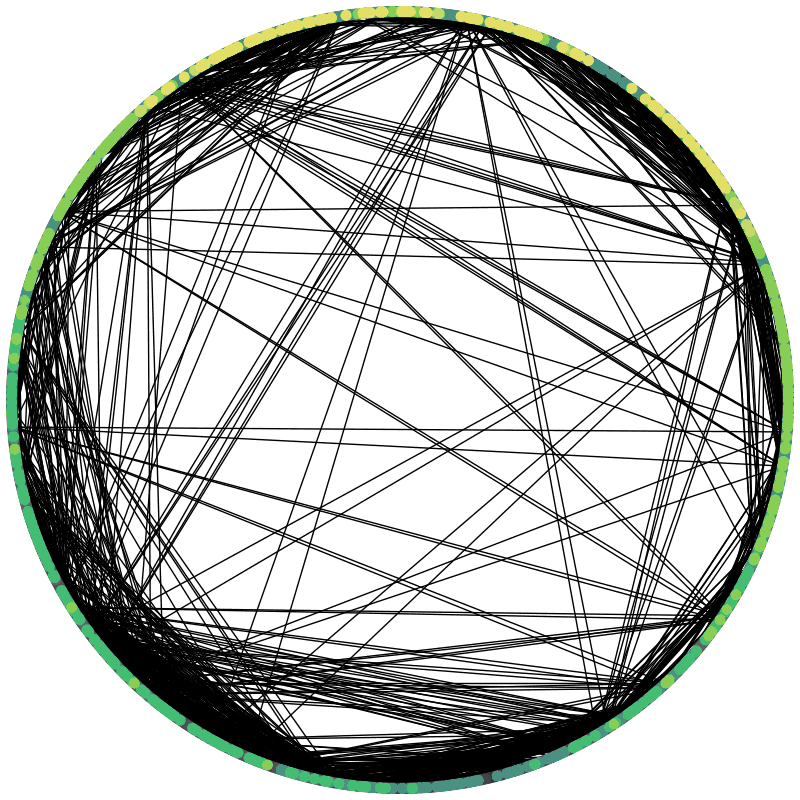
\includegraphics[width=0.175\columnwidth]{circle/vis/dwt_992_SA-L-BFGS_50_first.png} & 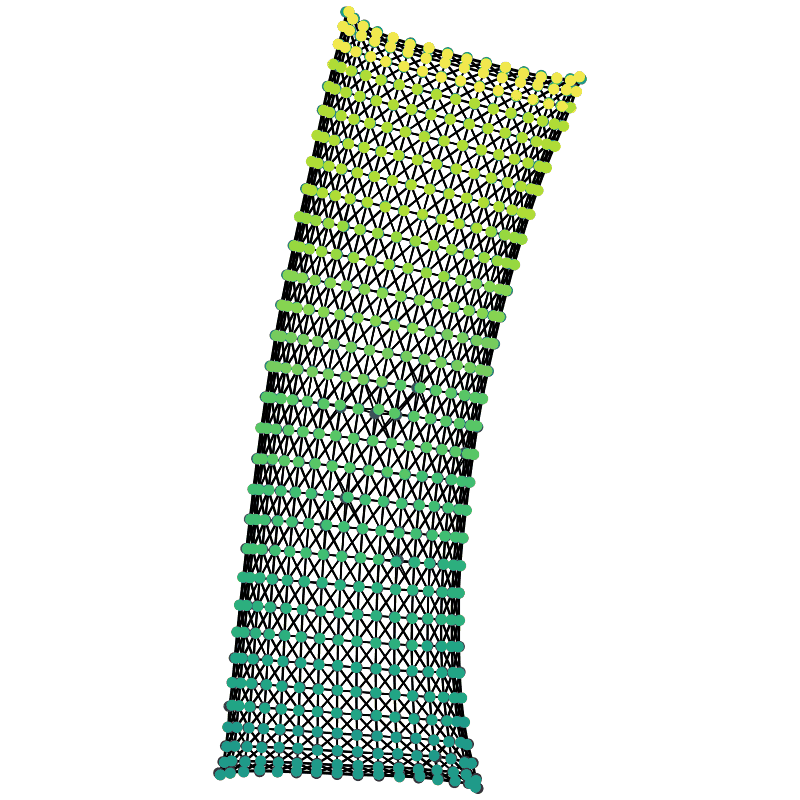
\includegraphics[width=0.175\columnwidth]{circle/vis/dwt_992_SA-L-BFGS_50_last.png} & 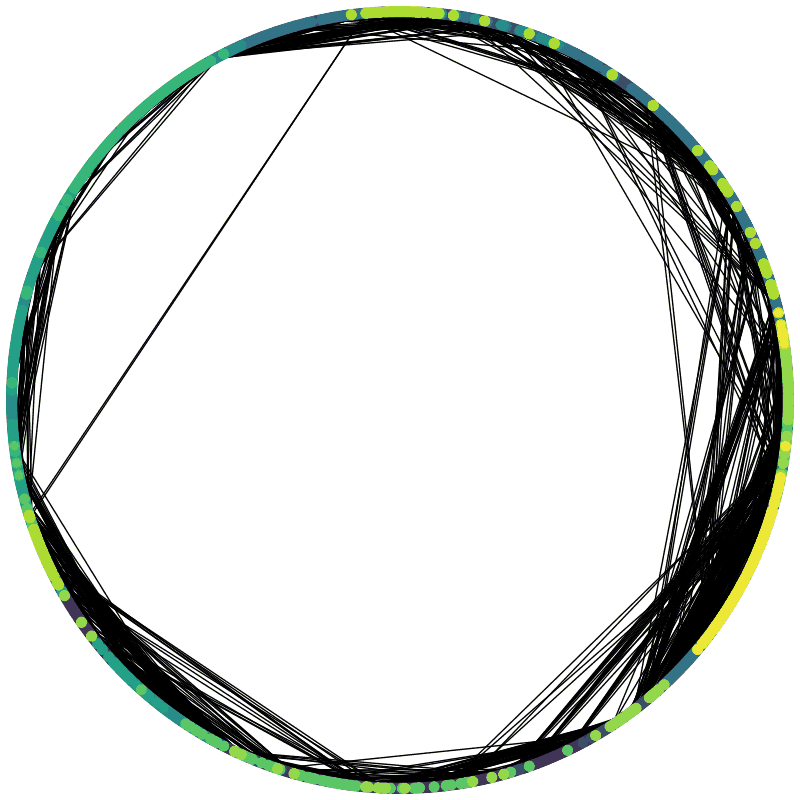
\includegraphics[width=0.175\columnwidth]{circle/vis/collins_15NN_SA-L-BFGS_50_first.png} & 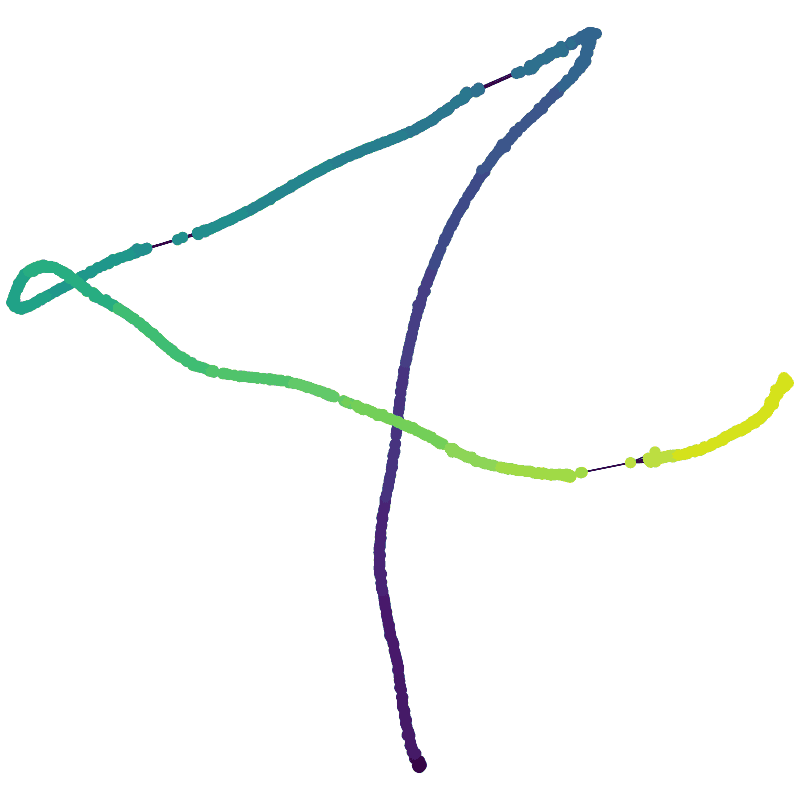
\includegraphics[width=0.175\columnwidth]{circle/vis/collins_15NN_SA-L-BFGS_50_last.png}   \\
    \addlinespace \rotatebox{90}{\quad \textsf{CN} (proposed)}              & 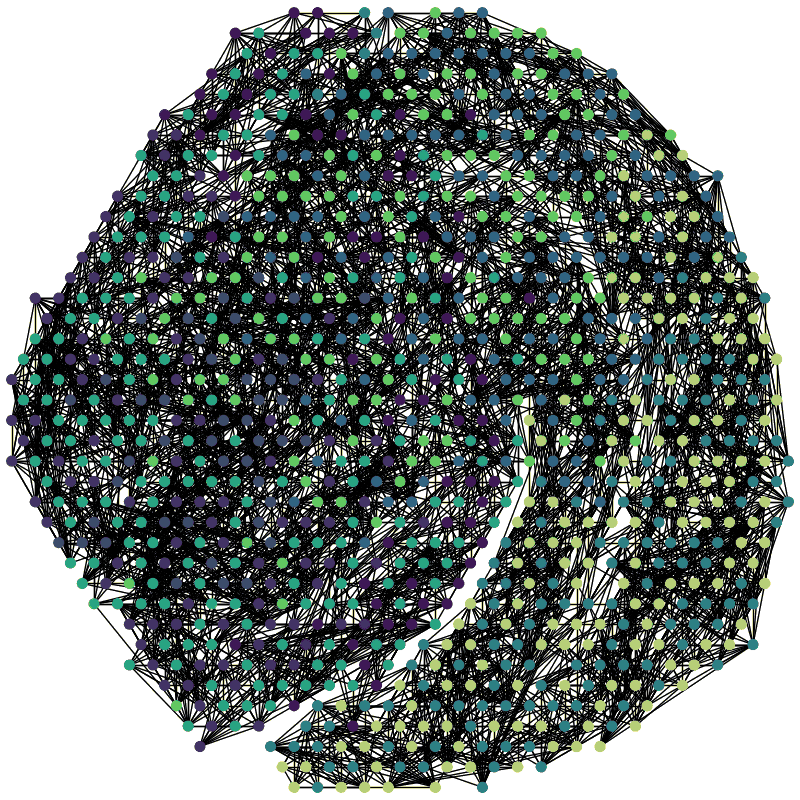
\includegraphics[width=0.175\columnwidth]{circle/vis/dwt_992_CN-L-BFGS_50_first.png} & 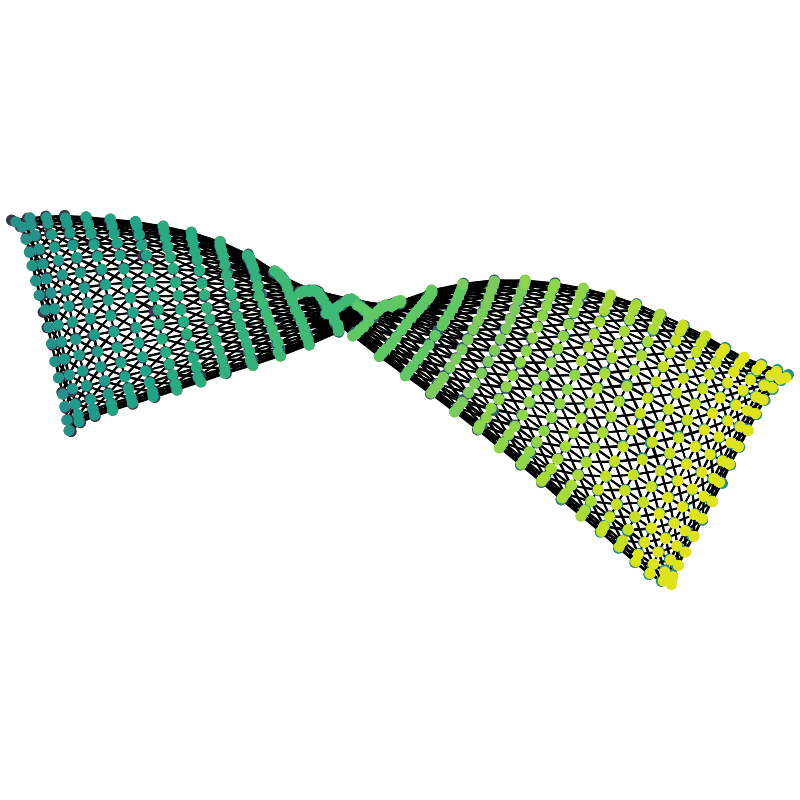
\includegraphics[width=0.175\columnwidth]{circle/vis/dwt_992_CN-L-BFGS_50_last.png} & 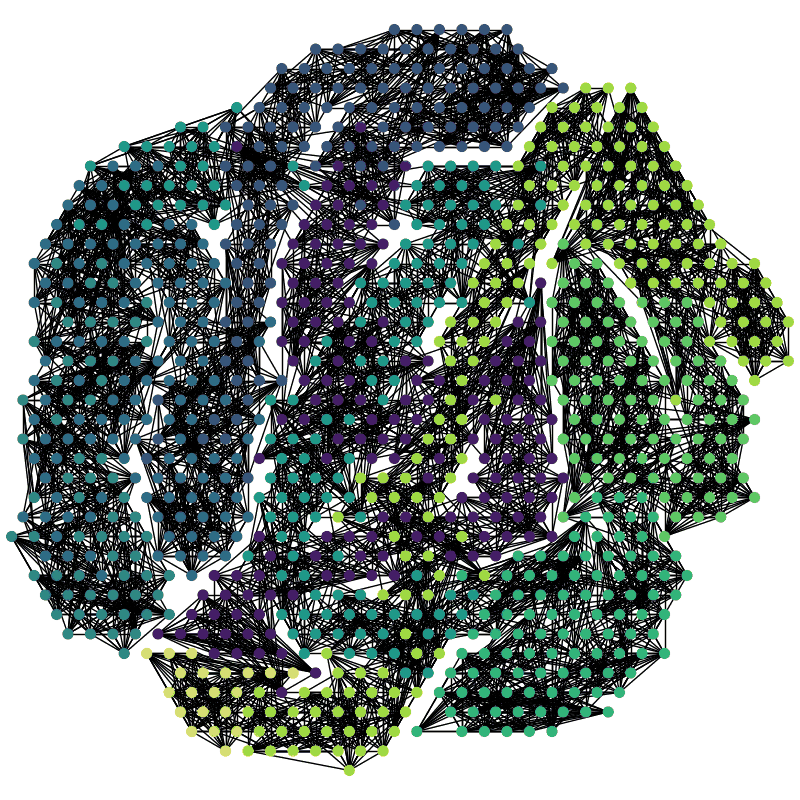
\includegraphics[width=0.175\columnwidth]{circle/vis/collins_15NN_CN-L-BFGS_50_first.png} & 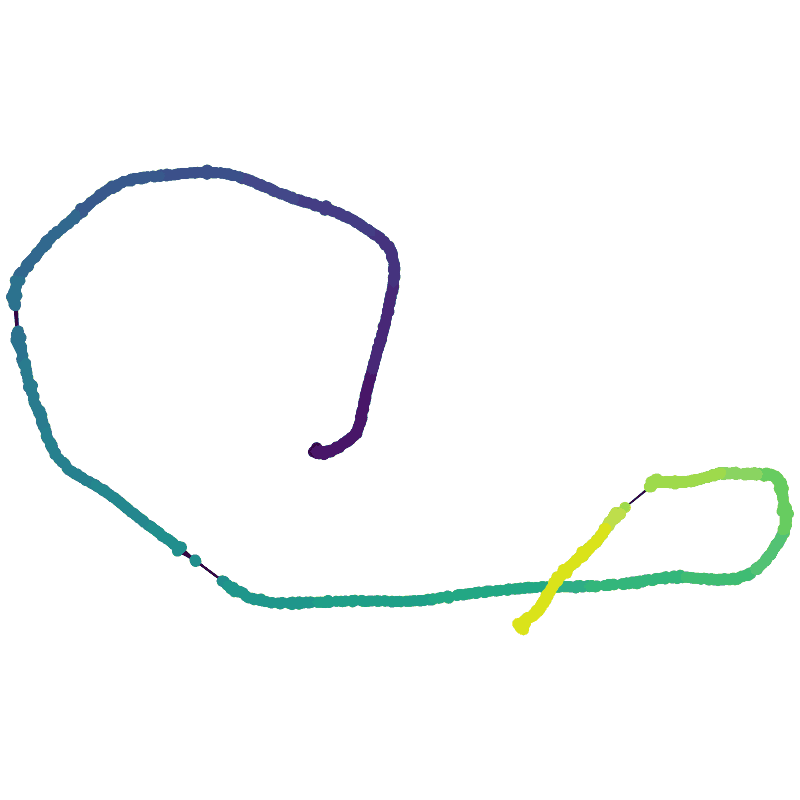
\includegraphics[width=0.175\columnwidth]{circle/vis/collins_15NN_CN-L-BFGS_50_last.png}   \\
    \bottomrule
  \end{tabular}
  \caption{Visualization results showing initial and 50th iteration placements
    for \texttt{dwt\_992} and \texttt{collins\_15NN}.}
  \label{fig:CN_vs_SA}
\end{figure*}

Next, we conducted experiments to evaluate the performance of the proposed algorithm
(\textsf{CN}) compared to random initialization (no prefix) and SA
initialization (\textsf{SA}) with various graphs.

We used all undirected, connected, non-negative weighted graphs with $1{,}000$
or fewer vertices, which can be generated using the matrices from the Sparse
Matrix Collection~\citep{davisUniversityFloridaSparse2011} as adjacency matrices. For
fairness, when we compare with \textsf{SA}, we converted the graphs to an unweighted
one. It means that we set weights $a_{i,j}$ to $1$ if $a_{i,j}> 0$; otherwise,
we set it to $0$.

For the algorithms with random initial placement, we set $N_{\mathrm{iter}}^{\mathsf{FR}}
  = N_{\mathrm{iter}}^{\red{\mathsf{LBFGS}}}= 50$ , the same as the default parameter
in NetworkX~\citep{hagbergExploringNetworkStructure2008}. For the \textsf{CN} algorithms, we set
$N_{\mathrm{iter}}^{\mathsf{FR}}= N_{\mathrm{iter}}^{\mathsf{LBFGS}}= 45$,
since the preprocessing step is expected to take as long as a few iterations
of FR or L-BFGS, as mentioned in \cref{ssec:setup}.

The results are shown in \cref{fig:overall,fig:diff}. The proposed algorithm
performed better than random or SA initialization, except for a few cases. As
for random initialization, one of such bad cases is \texttt{Spectro\_10NN}
shown in \cref{fig:proposeIsBad}. The proposed algorithm failed to resolve the
twist in the initial placement, shown in the figure, leading to a worse result.
Still, the average performance of ten seeds for \texttt{Spectro\_10NN} was almost the same as that of the random initialization. \Cref{fig:CN_vs_SA} provides examples for comparison with SA initialization. The proposed algorithm outperformed in \texttt{collins\_15NN} and underperformed in \texttt{dwt\_992}.

The interpretation of the results is as follows. First, results in
\cref{fig:overall,fig:diff} strongly support the effectiveness of the proposed
algorithm. It successfully untangles the twists, leading to better outcomes
with faster convergence. Even when the proposed algorithm performed worse, the
difference was insignificant in almost all cases. Secondly, the structural
difference between the initial placement and the optimal placement potentially
affects the convergence speed. For example, the optimal shape of \texttt{collins\_15NN}
is linear, differing from a circle, resulting in \textsf{SA}'s performance
being inferior to the proposed algorithm, whereas the opposite holds for \texttt{dwt\_992}.
Although the proposed method utilizes a hexagonal lattice $Q^{\mathrm{hex}}$,
alternatives such as $Q^{\mathrm{circle}}$ may lead to improved performance of
the proposed method in some cases.

Furthermore, although this is a case not considered in Ref.~\citep{ghassemitoosiSimulatedAnnealingPreProcessing2016}, we also conducted experiments with \textsf{CN} and \textsf{SA} for a case where the edge weight $a_{i,j}$ is not necessarily in $\qty{0,1}$.
We generated a weighted graph with 100 vertices in three groups and 1000 edges randomly, and if the two vertices were in the same group, we set the edge weight to $1.0$; otherwise, we set it to $0.1$.
It exhibits both strong and weak connections.
\Cref{fig:weightedDense} shows the difference between the two initializations.
When we ignore the edge weights and just solve the problem~\eqref{eq:sa}, the graph is just an Erd\H{o}s--R\'enyi graph, and thus \textsf{SA} cannot find any meaningful structure in the initial placement.
In contrast, the proposed algorithm can identify the graph's structure, and we can observe that the left graph in \cref{fig:weightedDense} is separated into groups, as indicated by the node colors.
This result suggests that our proposed algorithm is effective even for weighted graphs, extending the applicability of the preprocessing step.

\section{Rationale for the Discretization Approach}
\label{sec:rationale}

This section explains why we did not apply the coordinate Newton direction technique directly to the original problem~\eqref{prob:fr}, but instead first transformed it into the discrete optimization problem~\eqref{eq:frApprox0}.
At first sight, one might expect that applying the coordinate Newton method directly to~\eqref{prob:fr} would be more natural and possibly more efficient, since it avoids the detour through discretization. However, as we shall see, this approach suffers from intrinsic difficulties that undermine its effectiveness.
By contrast, our discretization-based formulation allows us to circumvent these difficulties while still exploiting the advantages of the coordinate Newton direction. This not only justifies our methodological choice but also provides a foundation for exploring further optimization strategies built upon this framework. In what follows, we clarify the limitations of the direct approach and explain how our method addresses them.

\subsection{Possible Alternatives}
\label{ssec:possibleApproach}

One natural idea for solving problem~\eqref{prob:fr} is to apply existing optimization algorithms such as Stochastic Gradient Descent (SGD) or Stochastic Coordinate Descent.

Applying SGD to graph drawing, particularly to the Kamada–Kawai (KK) layout~\citep{kamadaAlgorithmDrawingGeneral1989}, has been a notable direction~\citep{zhengGraphDrawingStochastic2019,ahmedMulticriteriaScalableGraph2022a}. The KK model determines the layout by minimizing a stress-like energy $\Phi_{i,j}^{\mathrm{KK}}$ defined for all vertex pairs. SGD corresponds to randomly selecting an edge ${i,j}$ and updating $x_i$ and $x_j$ using the gradient of $\Phi_{i,j}^{\mathrm{KK}}$. This stochastic treatment reduces per-iteration complexity while retaining structural information, as $\Phi_{i,j}^{\mathrm{KK}}$ is defined in terms of graph distance.

In contrast, applying SGD directly to the FR model is ineffective. When $a_{i,j}=0$, the energy term reduces to $\Phi_{i,j}=-k^{2}\log d$, which depends only on Euclidean distance and ignores the graph structure. Consequently, gradients from a single sampled pair often fail to provide meaningful information for optimization.

Another approach is to use Stochastic Coordinate Descent, which resembles Randomized Subspace Newton methods~\citep{NEURIPS2019_bc6dc48b, fujiTheoreticalAnalysisRandomized2025, cartisRandomisedSubspaceMethods2022, nozawaRandomizedSubspaceGradient2023, higuchiFastConvergenceSecondOrder2024}.
For each vertex $i$, define the local energy
\begin{equation}\label{eq:fi}
  \Phi_{i}(x_{i}) \defeq \sum_{j \in V \setminus \{i\}}\Phi_{i,j}(\norm{x_i - x_j}),
\end{equation}
whose gradient (the net force on $i$) and Hessian are
\begin{gather*}\label{eq:gradientFi}
  \nabla \Phi_{i}(x_{i}) = \sum_{j \in V \setminus \{i\}} \qty(\frac{a_{i,j}\norm{x_i - x_j}}{k}- \frac{k^{2}}{\norm{x_i - x_j}^{2}}) (x_{i}-x_{j}),\\
  \nabla^{2}\Phi_{i}(x_{i}) = \sum_{j \in V \setminus \{i\}}\left(\frac{a_{i,j}\norm{x_i - x_j}}{k} - \frac{k^{2}}{\norm{x_i - x_j}^{2}}\right) \mqty(1&0\\0&1)+ \\
  \sum_{j \in V \setminus \{i\}}\left(\frac{a_{i,j}}{k \norm{x_i - x_j}}+ \frac{2k^{2}}{\norm{x_i - x_j}^{4}}
  \right) (x_{i}- x_{j})(x_{i}- x_{j})^{\top}.
\end{gather*}
A direct SCD scheme randomly selects a vertex $i$, applies Newton’s method (or a regularized variant) to $\Phi_{i}$ using the above gradient and Hessian, and updates $x_{i}$ iteratively until convergence.

Although reasonable in spirit, this approach is also ineffective in practice. In the following, we illustrate the reasons for this failure with nontrivial examples.

\begin{figure}[t]
  \centering
  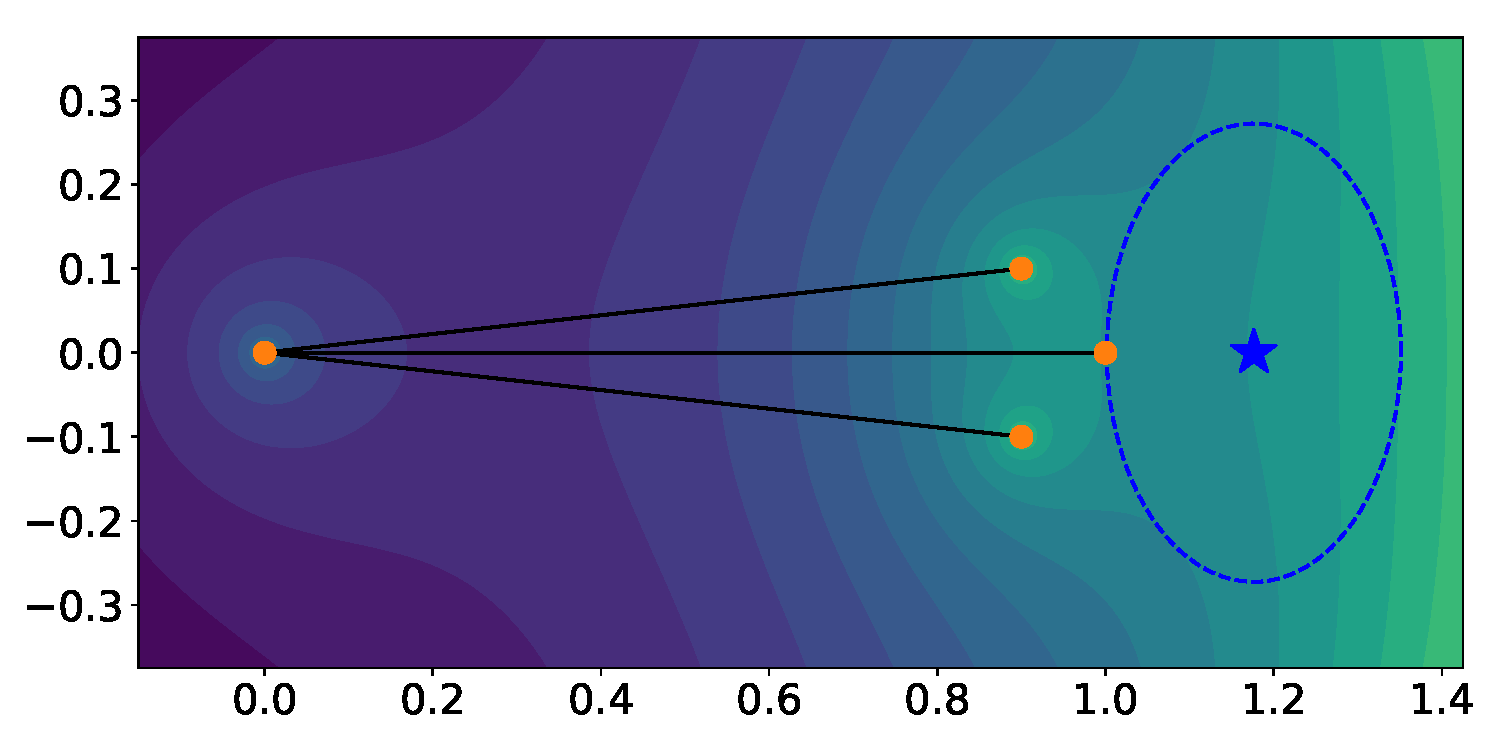
\includegraphics[width=0.8\columnwidth]{whyRSNfail1/whyRSNfail1.pdf}
  \caption{ The inaccurate quadratic approximation. The blue star indicates
    the optimal solution for the quadratic approximation of $\Phi_{1}(x_{1})$, but this
    differs significantly from the situation shown by the contour lines. }
  \label{fig:whyRSNfail}
\end{figure}

\subsection{Inaccuracy of Quadratic Approximation}
\label{ssec:inaccuracy}

One of the reasons it fails is the inaccuracy of the quadratic approximation; specifically, a particular issue arises when we restrict the optimization to a coordinate block.

Let $G$ be a graph with $V = \{1, 2, 3, 4\}$ and $E = \{\{1, 2\}, \{2, 3\}, \{2
  , 4\}\}$. Set $k = 1/2$ and assign all positive edge weights $a_{i,j}= 1$ for
every edge in $E$. The position of the vertices is
\begin{equation*}
  X =
  \begin{pmatrix}
    1 & 0 & 0.9  & 0.9  \\
    0 & 0 & +0.1 & -0.1
  \end{pmatrix}.
\end{equation*}
We show the contour of $\Phi_{1}(x_{1})$ in \cref{fig:whyRSNfail}.
The key point of this example is that the Hessian
\begin{equation*}
  \nabla^{2}\Phi_{1}(x_{1}) = \mqty(4.25&0 \\
  0&1.75)
\end{equation*}
is positive definite and well-conditioned.
Despite this favorable property of the Hessian, the coordinate Newton direction for $x_{1}$ results in a deviation from the global optimum.
This issue arises from the inaccurate approximation of $\Phi_{1}$ in the restricted block coordinates $x_{1}$.
The attractive force from vertex $2$ and the repulsive forces from vertices $3$ and $4$ cancel each other out, leading to a highly inaccurate quadratic approximation.
This deficiency cannot be entirely resolved by modifying Newton's method, as it is an intrinsic and unavoidable limitation of the stochastic coordinate descent.

\subsection{Ignorance of Other Vertices' Movements}
\label{ssec:ignorance}

Another reason is the ignorance of other vertices' movements when optimizing each vertex individually. When optimizing for a vertex $i$, the coordinate Newton direction treats all other vertices $V \setminus \{i\}$ as fixed.

\Cref{fig:whyRSNfail2} illustrates this issue. Consider a subset of vertices forming a mesh-like structure in $G$, where all vertices receive forces in the directions indicated by the blue arrows. In this situation, the FR and L-BFGS algorithms move all vertices simultaneously, allowing the simulation or optimization to proceed without issues. In contrast, the stochastic coordinate descent, as shown on the right side of the figure, brings stagnation. Here, all other vertices are considered fixed. Thus, optimizing the red vertex results in minimal movement,
as its directly connected neighbors impede it. As a result, even after
numerous iterations, little optimization is achieved. Thus, ignoring the movements of other vertices can be a significant limitation of the coordinate Newton method.

\begin{figure}[t]
  \centering
  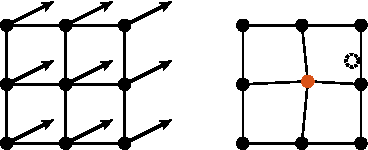
\includegraphics[width=0.6\columnwidth]{whyRSNfail2/whyRSNfail2.pdf}
  \caption{ The blue arrows represent the acting forces in this situation. The center vertex exhibits only a minor shift in the coordinate Newton direction, while the red dashed vertex marks its ideal configuration. }
  \label{fig:whyRSNfail2}
\end{figure}

\subsection{Rationale for Proposed Method}
\label{ssec:rationale}

Our proposed method resolves issues in \Cref{ssec:inaccuracy,ssec:ignorance} by transforming the problem~\eqref{prob:fr} into the problem~\eqref{eq:frApprox0}
in \cref{ssec:reduction}, and optimizing $\Phi^{\mathrm{a}}_{i}$ on $Q^{\mathrm{hex}}$.

Regarding the issue in \cref{ssec:inaccuracy}, this transformation brings the convexity of the objective function as it treats the repulsive forces via a hexagonal lattice, making the quadratic approximation more accurate than the original problem.
Regarding the issue in \Cref{ssec:ignorance}, the discrete point set $Q$ ensures that the stepsize is larger than $\epsilon$, as each point is always separated by at least $\epsilon$. This large stepsize prevents
stagnation in the optimization, and helps explore the solution space more efficiently.
Furthermore, this transformation also brings the benefit of reducing computational complexity from $\order*{\abs{V}^2}$ to $\order{\abs{E}}$.

Thus, converting the problem is crucial to provide a high-quality initial
placement with the coordinate Newton direction. There may also be better transformation methods, and further exploration is warranted.

\section{Conclusion}\label{sec:conclusion}

In this study, we proposed a new initial placement with the coordinate Newton
direction for the FR force model, the problem~\eqref{prob:fr}. % LLDisable
The obtained initial placements have fewer twists than the random initialization, leading to faster convergence and better visualization.
Numerical experiments revealed that the proposed method is effective across various graphs, extending the applicability of the preprocessing step.
The proposed method may advance the graph drawing, and we also hope it highlights the potential of the stochastic coordinate descent and its variants for addressing a broader range of graph-related optimization problems.

\section*{Acknowledgment}

We want to express our sincere gratitude to PL Poirion and Andi Han
for their insightful discussions, which have greatly inspired and influenced this research. We also thank the developers of NetworkX and Graphviz. Their excellent work has been a great help in conducting this research.

This work was partially supported by JSPS KAKENHI (26KJ0936, 23H03351, 24K23853) and JST ERATO (JPMJER1903).


\bibliographystyle{abbrvurl}
\bibliography{FruchtermanReingoldByRandomSubspace}

\appendix

\section{NetworkX Implementation}
\label{sec:algToProb1}

As supplementary information, this section explains how to solve the problem~\eqref{prob:fr} and obtain the final placement.
At the time of writing, NetworkX, an open-source library for graph analysis in Python, is set to release the L-BFGS-based method that we have implemented. Although this method does not use our proposed initial placement, we provide some implementation details as a reference in \cref{subsec:networkX_impl}.

\subsection{Fruchterman--Reingold Algorithm}
\label{ssec:frAlgorithm}

\begin{algorithm}[H]
  \caption{Fruchterman--Reingold algorithm}
  \label{alg:fr} \KwIn{Graph $G = (V, E)$, Weights $(a_{i,j})_{\{i,j\} \in E}$, Parameters $N_{\mathrm{iter}}^{\mathsf{FR}}\in \bbN$, $t_{0}> 0$, and Initial~placement~$X = (x_{1}, \dots, x_{n})$}
  \KwOut{Final placement $X$}

  $t \gets t_{0}$\; \For{$m \gets 1$ \KwTo $N_{\mathrm{iter}}^{\mathsf{FR}}$}{ $\text{compute gradient }\nabla \Phi_{i}(x_{i})$ for all $i \in V$\; $x_{i}^{\mathrm{new}}\gets x_{i}- t \frac{\nabla \Phi_{i}(x_{i})}{ \norm{\nabla f_i(x_i)}}$ for all $i \in V$\; $x_{i}\gets x_{i}^{\mathrm{new}}$\; $t \gets t - t_{0}/ N_{\mathrm{iter}}^{\mathsf{FR}}$\; \If{\text{convergence condition is satisfied}}{ \textbf{break}\; } }
  \Return $X$\;
\end{algorithm}

The Fruchterman--Reingold algorithm~\citep{fruchtermanGraphDrawingForcedirected1991} is the original and most standard approach to obtain the equilibrium state of the force model.
The pseudo-code is shown in \cref{alg:fr}, which is a variant of the gradient (steepest) descent method with the function $\Phi_{i}$ in \cref{eq:fi}~\citep{tunkelang1999numerical}.

\Cref{alg:fr} is based on the original pseudo-code~\citep{fruchtermanGraphDrawingForcedirected1991} and implementation in NetworkX~\citep{hagbergExploringNetworkStructure2008} with some omitted details.
We typically draw the initial placement $X$ from a uniform distribution on $[0,1]^{2 \times n}$.
The parameter $t$ denotes the temperature, which governs the stepsize along the steepest descent.
As the temperature gradually decreases, the algorithm converges to a particular placement, which is not necessarily a local optimum of the problem~\eqref{prob:fr}.

\subsection{L-BFGS Algorithm}
\label{ssec:lbfgs}

\begin{figure}[t]
  \centering
  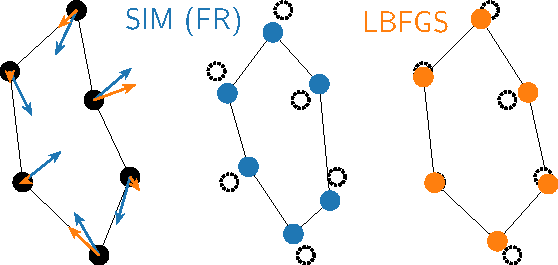
\includegraphics[height=3.59cm]{comparison/comparison_FRandLBFGS.pdf}
  \caption{Comparison of the FR and L-BFGS algorithms. Blue arrows represent fixed stepsizes in FR, whereas orange arrows represent adaptive stepsizes determined by the approximate inverse Hessian}
  \label{fig:comparisonFRandLBFGS}
\end{figure}

Another approach is to leverage the L-BFGS algorithm~\citep{6183577}. Using only
a few recent gradient vectors, the L-BFGS algorithm approximates the inverse
Hessian of the objective function $\Phi$~\citep{liuLimitedMemoryBFGS1989a}. L-BFGS
is known to be very efficient for large-scale optimization problems. We can apply
the L-BFGS algorithm to the optimization problem~\eqref{prob:fr} via flattening
the matrix $X \in \bbR^{2 \times n}$ to a vector $\overline{X}\in \bbR^{2n}$. Refer
to \cref{fig:comparisonFRandLBFGS} for a comparison to the FR algorithm.

\subsection{NetworkX Implementation}
\label{subsec:networkX_impl}

\begin{figure}[t]
  \centering
  
\includegraphics[width=\columnwidth]{networkx/fig1.png}
  \caption{ The FR algorithm and L-BFGS algorithm in NetworkX. }
  \label{fig:networkx1}
\end{figure}

In this subsection, we explain the details of our NetworkX implementation. Refer
to \cref{fig:networkx1} for a comparison to the FR algorithm. The problem
setting considered in NetworkX is similar to that described in~\cref{sec:preliminaries},
but there are some key differences. First, the number of dimensions is not always two. Since the extension of the method is straightforward, we restrict our discussion to two-dimensional layouts. Other than that, the following differences exist:
\begin{enumerate}[label=\textbullet, itemsep=0pt, parsep=0pt]
  \item Negative edge weights are allowed.

  \item Directed graphs are supported, not just undirected graphs.

  \item The graph is not always connected.
\end{enumerate}

Under these settings, the problem~\eqref{prob:fr} can be unbounded. It means
that the optimal solution does not exist in a finite region. When edge weights
are negative or the graph is disconnected, i.e., when it consists of $m >1$
connected components ($V=\bigoplus_{j=1}^{m}V_{j}$), the solution may be unbounded,
since the farther apart the vertices are, the lower the energy.

To overcome this issue, we do the following suitable modifications. First, when the graph has negative edge weights, one may transform them into non-negative values, for example, by taking their absolute values. Second, when the graph is a directed one, only the sum $a_{i, j}+ a_{j, i}$ matters in the formulation, so symmetrization is sufficient. Thus, the directed and possibly negatively weighted adjacency matrix $\Tilde{A}= (\Tilde{a}_{i,j}) \in \mathbb{R}^{n \times n}$ can be transformed into a symmetric matrix $A = (a_{i,j})$, where $a_{i,j}= (\lvert \Tilde{a}_{i,j}\rvert + \lvert \Tilde{a}_{j,i}\rvert)/2 \geq 0$. Third, we add additional forces to the energy function to prevent the divergence of each connected component. In general, adding terms that attract each group to the center is a common approach to avoid unboundedness. We adopt
this approach with the center $x_{\mathrm{center}}=(0.5, 0.5)^{\top}$, as it
is the center of the expected layout bounding box.

Based on \cref{sec:preliminaries}, let us define the sum of terms associated with the vertex $x_{i}$ be $\Phi_{i}$, which
is explicitly given by
\begin{equation*}
  \Phi_{i}(x_{i}) \coloneqq \sum_{j \in V \setminus \{i\}}\left( \Phi_{i,j}(\norm{x_{i}- x_{j}}
  ) + \Phi_{j,i}(\norm{x_{j}- x_{i}}) \right).
\end{equation*}
The $i$-th row of the gradient $\nabla \Phi(X) \in \mathbb{R}^{2 \times n}$ is
\begin{align*}
  (\nabla \Phi(X))_{i}^{\top} & = \nabla \Phi_{i}(x_{i}) = \sum_{j \in V \setminus \{i\}}\left(\frac{(a_{i,j}+a_{j,i})\norm{ x_{i}- x_{j}}}{k}- \frac{2k^{2}}{\norm{ x_{i}- x_{j}}^{2}}\right) (x_{i}- x_{j}) \\
                           & = 2 \sum_{j \in V \setminus \{i\}}\left(\frac{a_{i,j}\norm{ x_{i}- x_{j}}}{k}- \frac{k^{2}}{\norm{ x_{i}- x_{j}}^{2}}\right) (x_{i}- x_{j}).
\end{align*}
To obtain the final layout while preventing the divergence, we need to
minimize $\Phi(X) + f_{\mathrm{g}}(X)$, where $f_{\mathrm{g}}(X)$ is the additional
term. Let the center of gravity of the $j$-th connected component $V_{j}$ ($1 \leq
  j \leq m$) be $g_{j}\coloneqq \frac{1}{|V_{j}|}\sum_{i \in V_j}x_{i}$. Then,
using some constant $c_{\mathrm{g}}>0$, we define the additional force as
\begin{equation*}
  \Phi_{\mathrm{g}}(X) \coloneqq c_{\mathrm{g}}\sum_{j=1}^{m}\frac{\lvert V_{j}\rvert}{2}
  \norm{ g_{j} - x_{\mathrm{center}}}_{2}^{2},
\end{equation*}
with the gradient
\begin{equation*}
  (\nabla \Phi_{\mathrm{g}}(X))_{i}= c_{\mathrm{g}}(g_{j}- x_{\mathrm{center}}) \quad
  \text{where}\quad i \in V_{j}.
\end{equation*}
We can now apply the L-BFGS algorithm to these functions to derive the algorithm.
Further implementation details and experimental results are available in
\href{https://github.com/networkx/networkx/pull/7889}{our merged pull request}
to the NetworkX.

\end{document}
